%
% Chapter 3
%

\chapter{EXPERIMENTAL APPARATUS}

\section{The Large Hadron Collider}
The most powerful machine of its kind, the Large Hadron
Collider (LHC) accelerates and collides particles
at high center-of-mass energies producing rare
particles and interactions that would be otherwise unobservable
in the laboratory, making it the best tool available for producing \tth
processes. The LHC is a circular particle accelerator/collider. Measuring 27 km
in circumference, it collides beams of protons in head-on collisions       
at a center-of-mass energy of 13 TeV.

Originally conceived in the early 1980s and approved in 1994, the LHC was designed to replace the then-operating
Large Electron Positron Collider (LEP), re-using the same underground tunnel. Located just outside Geneva, Switzerland, at the Center for European Nuclear Research (CERN),
the LHC stretches across the border into France. There are four detector experiments positioned around the LHC: ALICE, ATLAS, CMS, and LHCb. The two general purpose,
functionally-equivalent detectors are ATLAS and CMS, while ALICE studies heavy ion collisions, and LHCb studies flavor physics. 
The motivation for having two equivalent detectors is to provide cross checks on results, as each result is produced with separate analysis teams, studying separate collsions
recorded with a separate detector. Each detector is centered on an interaction point, where the beams are steered into each other to produce collisions. 
The LHC itself is technically the final element in a series of accelerators
that bring particle beams from rest to succesively higher energies. This system of
of accelerators, referred to as the LHC Accelerator Complex is depicted below in
Figure~\ref{fig:lhc_complex}.

The acceleration is accomplished with radio frequency (RF) cavities. RF cavities are a linear series of cylindrical conductors,
which sustain a resonant electromagnetic field produced by a generator. As 
charged particles pass through the cavities, they experience a force
(acceleration) from the resonant alternating field in each cavity. This acceleration process begins with Hydrogen gas in the linear accelerator
(LINAC 2). The Hydrogen atoms in the gas are stripped of electrons
in an applied electric field, leaving only protons, which are then accelerated
along the linear beam pipe with RF cavities to an energy of 50 MeV. After the LINAC, the beams of protons enter the Proton Synchrontron Booster rings where
they are accelerated to 1.4 GeV, before reaching the Proton
Synchrotron (PS). The circular PS, measuring more than 600 m
in circumference, accelerates the beams to 25 GeV before injection into the
larger, Super Proton Synchrotron (SPS). The SPS at over 7 km around, provides the final
acceleration before the beams reach the LHC at an energy 450 GeV. The SPS injects the beams into
the LHC in opposite directions to facilitate collisions later. After the beams are fully injected, the LHC ramps the beam energy to 6.5 TeV per beam, providing 13 TeV center-of-mass proton collisions~\cite{lhc_bluebook}.

The beam pipes of the entire accelerator complex are kept at an ultra high vaccuum
to avoid detrimental beam interactions before the collisions. Since the beams are made up of protons which have electric charge,
they can be focused and steered around the LHC with 392 quadrupole and 1232 dipole superconducting magnets.
To accomplish this, the magnets produce a field of over 8 Tesla. This is possible thanks to the
superconducting niobium-titanium (NbTi) coils which are cooled with liquid nitrogren and superfluid helium-4. These
magnets operate at 1.9 K allowing them to carry a current of over 11000 amperes. In addition to
the LHC, superconducting magnets are used throughout the accelerator complex ~\cite{lhc_bluebook}.

Inside the LHC, the beams travel in opposite directions in separate but adjacent pipes inside of the superconducting magnets.
As a result of the RF cavity acceleration, the beams are comprised of individual 'bunches' of protons.
There are over 2800 bunches in each beam, with each bunch spaced 25 ns apart. This spacing is choosen to
produce as many bunch crossings as possible, without overloading
the detector instrumentation and data acquisition. There are approximately $10^{11}$ protons in each bunch, but due to the small cross section of the protons,
only approximately 20 collisions occur in each bunch crossing. The beams travel around the LHC over 11,246 times per second, over 99.99$\%$ the speed of light. 
This translates to around 600 million collisions per second ~\cite{lhc_bluebook}.

The center-of-mass energy and time-spacing between proton bunches in the LHC as well as a thorough understanding of them are critical to studying interesting
and rare physics processes like \tth. A sufficient center-of-mass collision energy is needed to produce new, heavy particles.
With the current center-of-mass collision energy of 13 TeV, any particle with mass less than or equal to this, is 
within reach of the LHC. Because many interesting physics processes are exceedingly rare (small cross section), many collisions
are needed. The quantity used to describe the rate of collisions is called Luminosity.
Described in equation~\ref{eqn:lumi_inst} below, instantaneous luminosity represents the number of collisions (events) occuring per unit time~\cite{lhc_bluebook}.

\begin{equation}
\label{eqn:lumi_inst}
\mathcal{L}_{inst} = \frac{N_{b}^{2}n_{b}f_{\textnormal{rev}}\gamma}{4\pi \epsilon_{n} \beta^{*}}F
\end{equation}

Where $N_{b}$ is the number of protons per bunch, $n_{b}$ is the total number of bunches, $f_{\textnormal{rev}}$ is the number of beam revolutions around the LHC per
second, $\gamma$ is a relativistic factor, $\epsilon_{n}$ is factor related to beam emittance, $\beta^{*}$ is the beta function representing the beam cross section, and
$F$ describes the factor related to the crossing angle of the beams. Because not every collision can be recorded, knowing the total number of collisions is critically important
to every analysis at an LHC collider experiment. From the instantaneous luminosity, the total number of collisions in time interval $t$, known as integrated luminosity
can be calculated by integrating over time in equation~\ref{eqn:num_coll} below. 

\begin{equation}
\label{eqn:num_coll}
N_{pp} = \int \sigma_{pp}\mathcal{L}_{inst}dt 
\end{equation}


\begin{figure}[hbtp]
 \begin{center}
   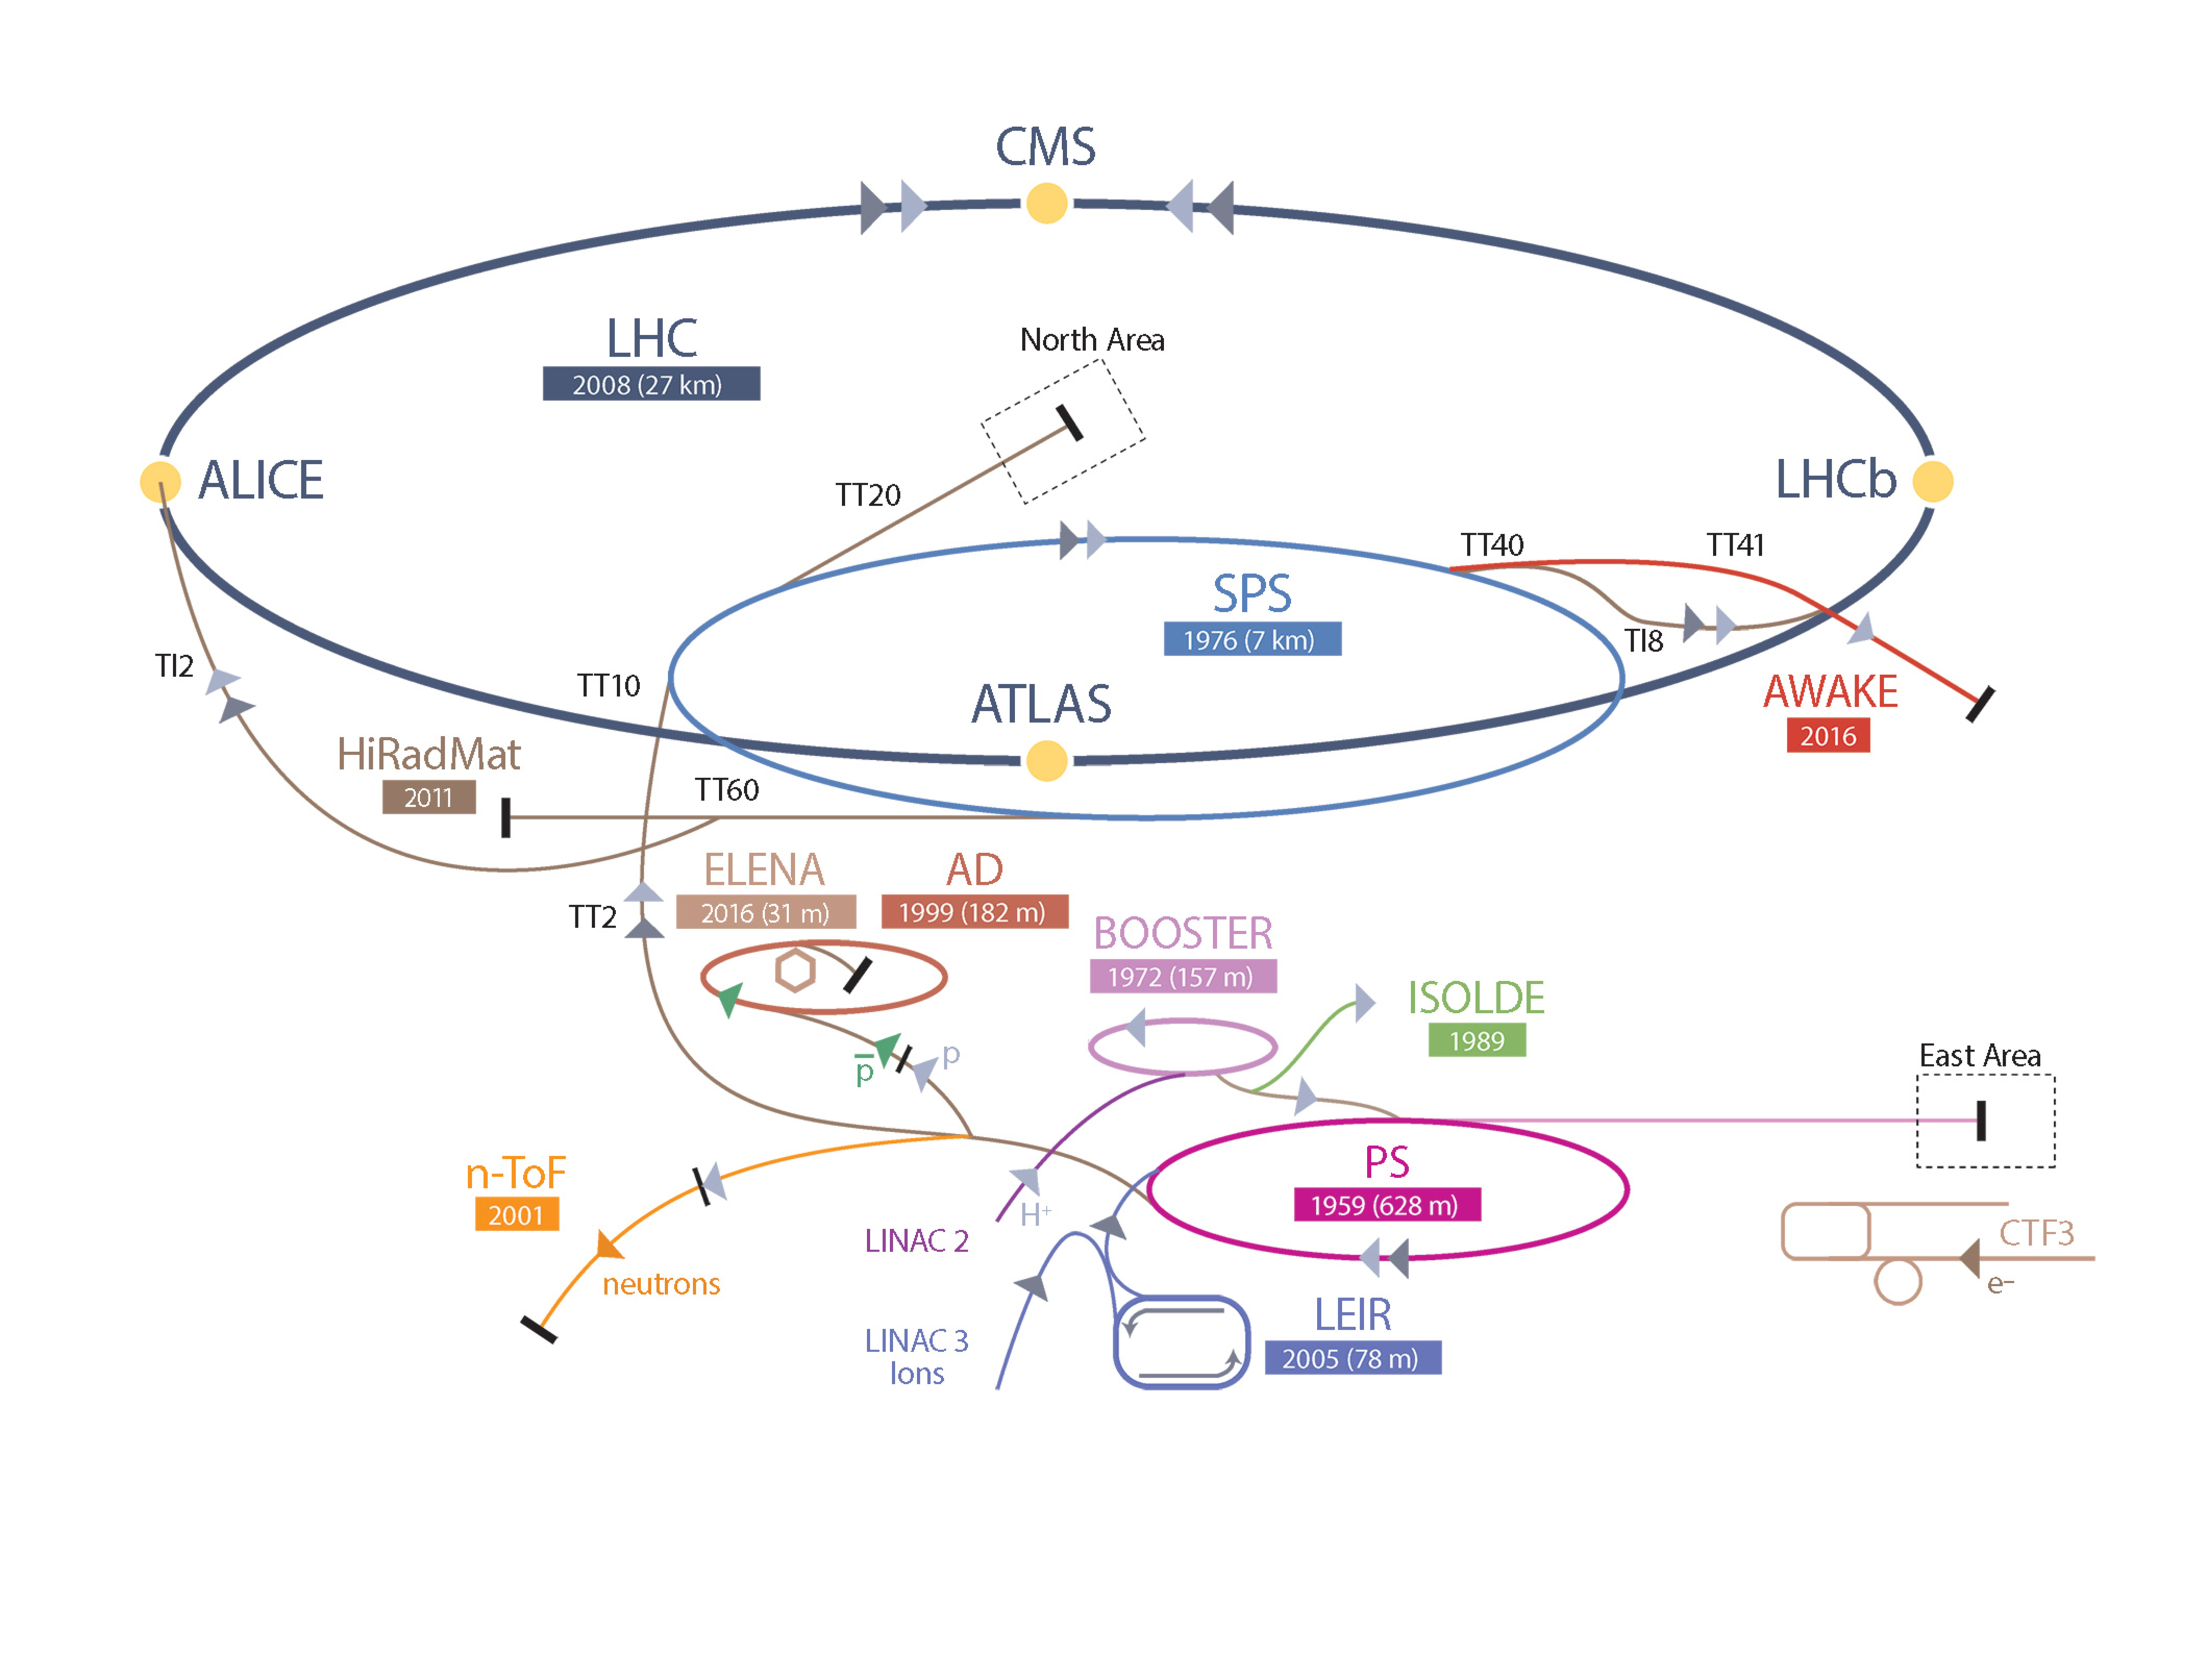
\includegraphics[width=0.9\textwidth]{ch3_figs/lhc_complex.pdf}
   \caption{An overview of the LHC accelerator complex~\cite{lhcfig}.}
   \label{fig:lhc_complex}
 \end{center}
\end{figure}


\section{The Compact Muon Solenoid (CMS) Detector}
The Compact Muon Solenoid (CMS) detector is a multi purpose particle detector designed to record and identify particles produced in collisions at the LHC, sitting 100 m underneath
the town of Cessy, France. CMS is comprised of layers of subdetectors which are connected to readout electronics and the trigger and data acquisition systems.
The various subdetectors record information about the collision, while the trigger and
data acquisition systems record and save the collisions. The acronym CMS comes from being more compact than its sister detector ATLAS, at 15 m in diameter and
over 21 m long. The name muon is because muons are the particles it detects with the greatest efficiency. The solenoid part of the name is due to the largest magnet of its kind
around which the detector is built. CMS is cylindrical in shape, as pictured in Figure~\ref{fig:cms_overview}. The various subdetectors and components are described in more
detail below. 

%% \begin{table}[hbtp]
%% \centering
%% \caption{Quantitative Summary of the CMS Detector}
%% \begin{tabular}{lcc}
%% \hline
%% Detector & Summary  \\
%% \hline
%% CMS total weight & 14000 tons  \\
%% %\hline
%% CMS diameter & 15.0 m \\
%% %\hline
%% neutralEmEnergyFraction (NEF)& \textless 0.99 \\
%% %\hline
%% neutralHadronEnergyFraction (NHF)& \textless 0.99 \\
%% %\hline
%% chargedHadronEnergyFraction (CHF) & \textgreater 0 \\
%% %\hline
%% number of charged hadrons (NCH) & \textgreater 0 \\
%% %\hline
%% N$_{constituents}$ & \textgreater 1 \\
%% \hline
%% \end{tabular}
%% \label{tab:JetTable}
%% \end{table}


\begin{figure}[hbtp]
 \begin{center}
   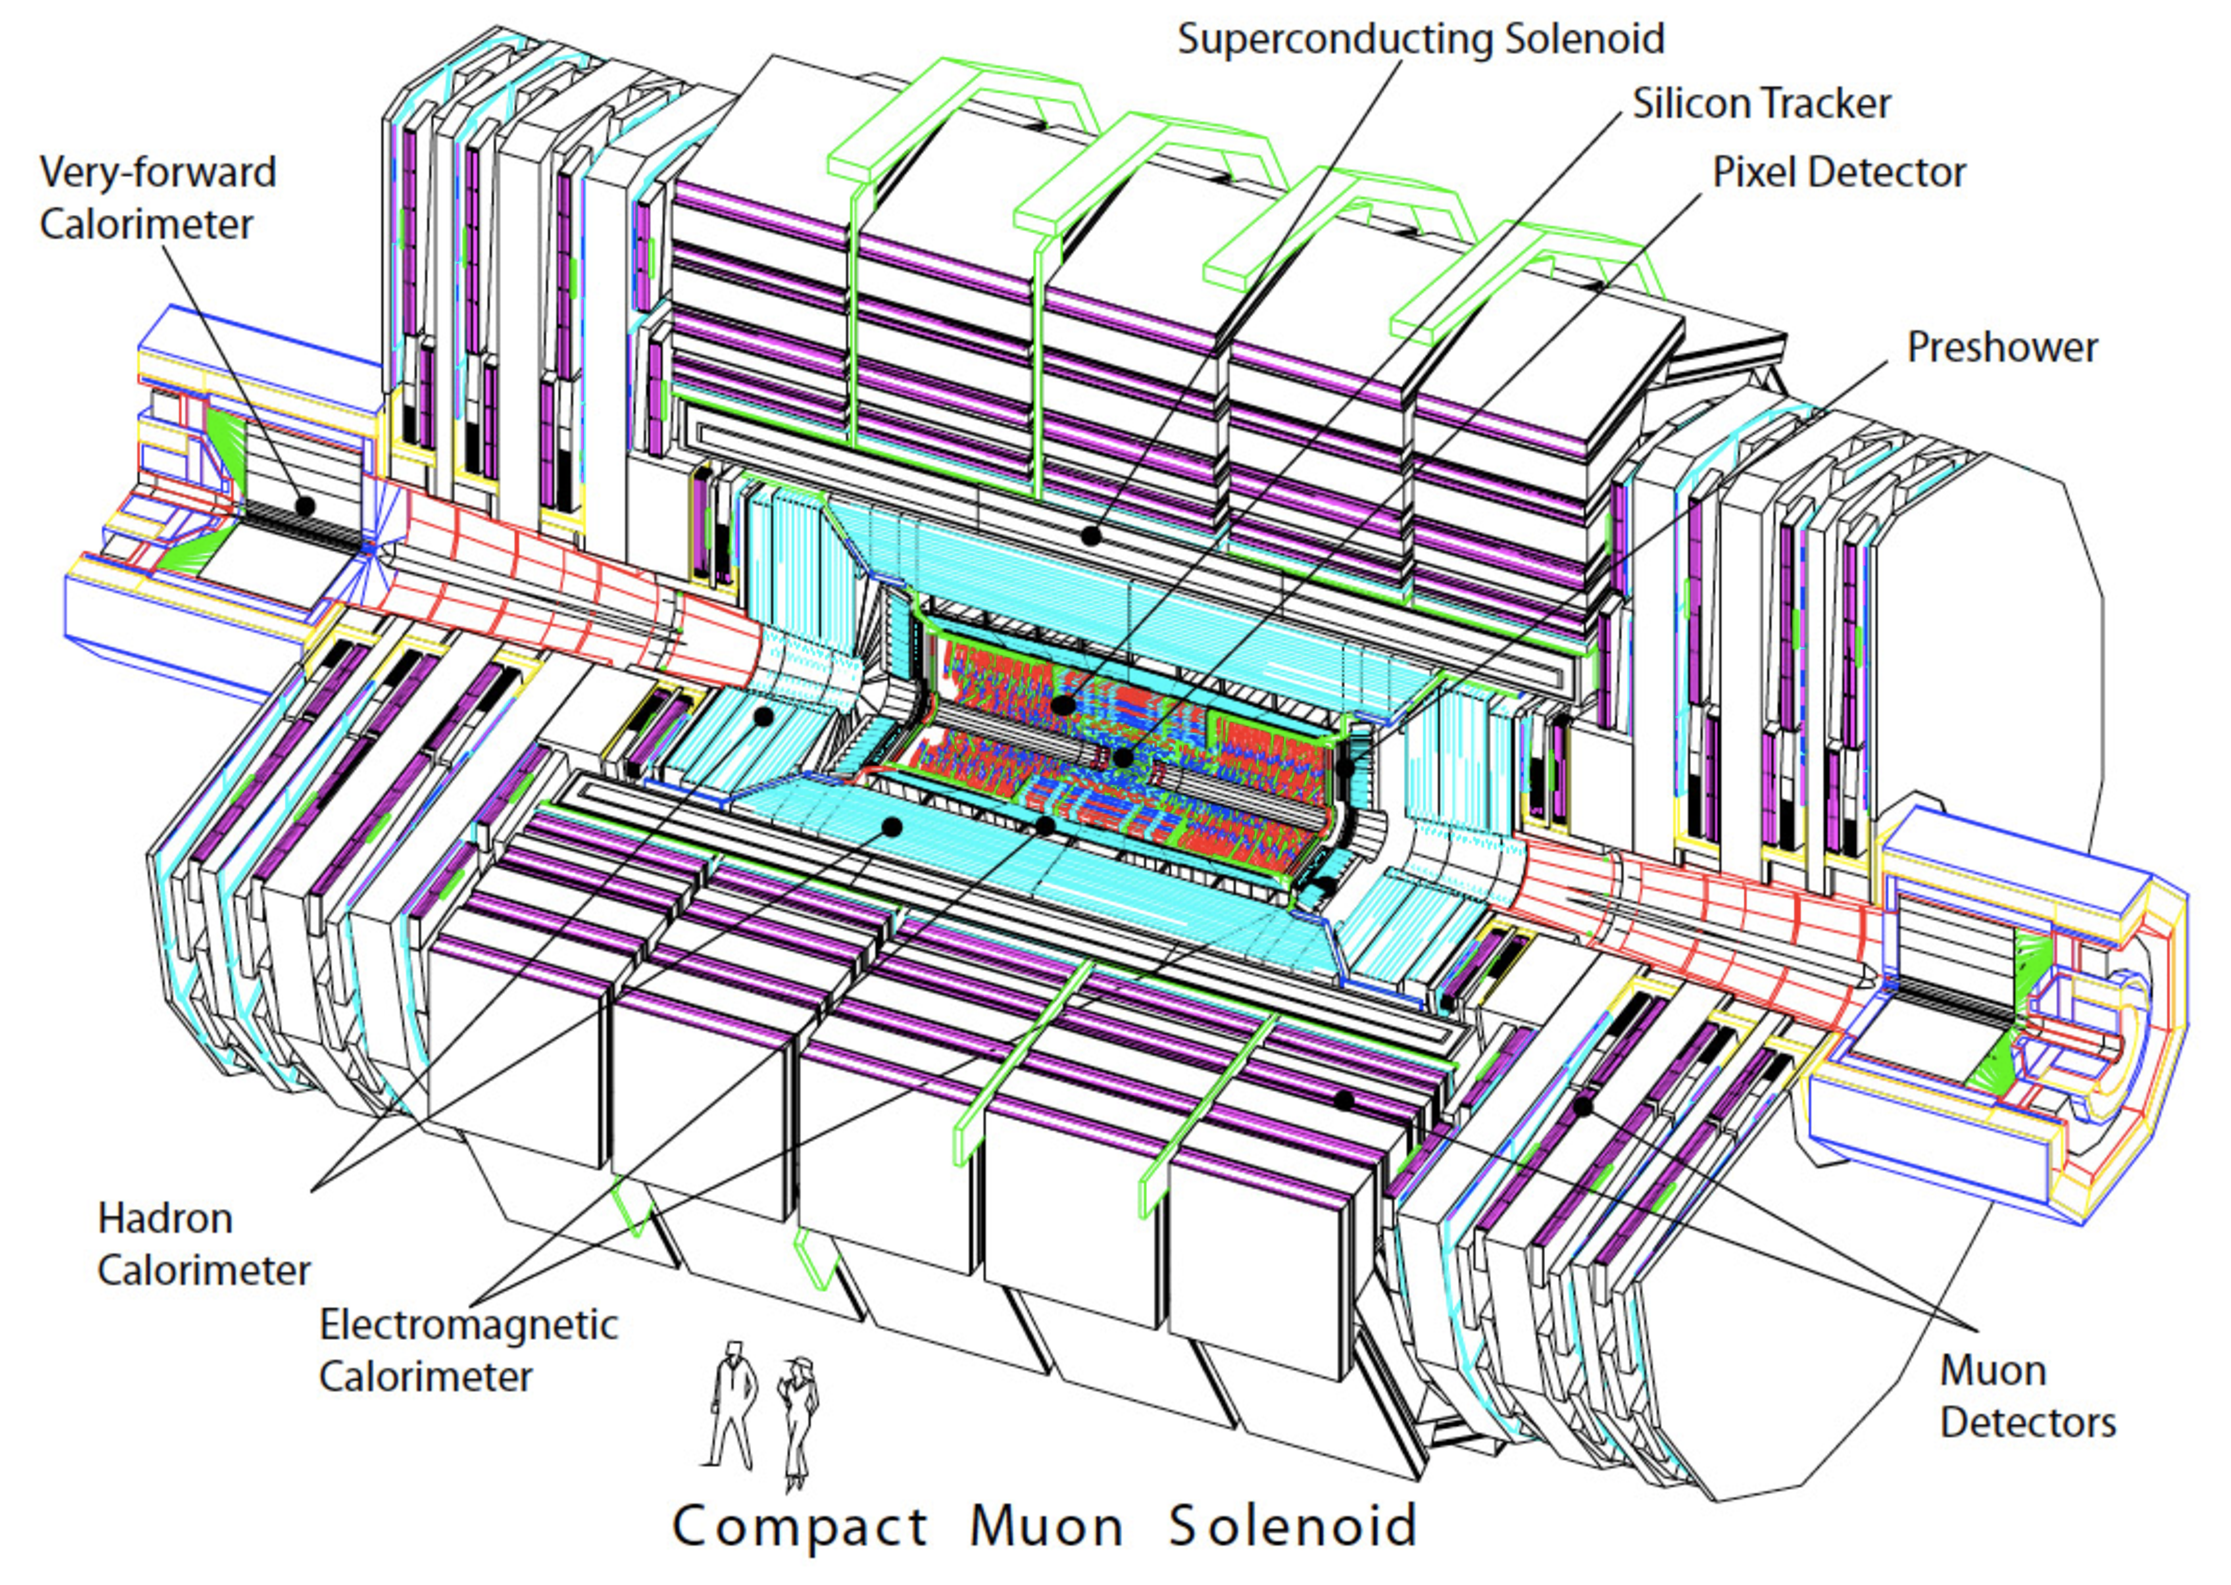
\includegraphics[width=0.9\textwidth]{ch3_figs/cms_overview_white.pdf}
   \caption{A qualitative overview of the CMS detector~\cite{cms_bluebook}.\label{fig:cms_overview}}
 \end{center}
\end{figure}

\subsection{Coordinate System}
Due to the geometry of the collisions produced inside CMS, a special coordinate system is used for simplicity. With the origin at the interaction point,
the y-axis in the vertical direction, the z-axis parallel to/along the beam direction, and the x-axis in the horizontal direction perpendicular to both the y
and z axes. In the transverse x-y plane, the angle formed with respect to the x-axis is $\phi$. In the y-z plane, the angle formed with respect to the z-axis
is $\theta$. The number of particles traveling through a given area, known as flux, increases towards the beam line, due to many more glancing collisons ocurring
than head-on collisions. The particles from the collisions are moving relativistically. Because of this, a special coordinate $\eta = -\ln\tan(\theta/2)$ 
is used to describe the angular position with respect to the z-axis, known as $pseudorapidity$. The head-on inelastic pp collisions have only momentum in the 
z-direction, thus measuring energy and momentum quantities in the transverse plane is important in analyzing and reconstructing collision events due to momentum
conservation.  

\subsection{Tracker}
\subsubsection{Pixel Detector}
The innermost piece of CMS is the tracking system, specifically the pixel detector. The pixel detector is comprised of 65 million silicon pixels, allowing it to record
precise trajectories of the charged particles resulting from collisions. Precise tracking information is critical to differentiating nearby particles, and identifying
exactly where an interesting collision took place. 

The pixel detector is about the size of a shoe box and contains 3 layers at 4 cm, 7 cm, and 11 cm from the beam.
The silicon material in the tracker is choosen specifically to disturb the particles as little as possible, while still providing accurate hit identification and track reconstruction.
Additionally, the material is resistant to radiation\footnote{Also known as radiation hard}, which is very important as it is only a few centimeters from the interaction point. Each silicon pixel measurses 100 $\mu$m by 150 $\mu$m. 

As the particles travel through successive layers of silicon pixels, they leave points of impact on each pixel, known as hits.
The hits are measured with a precision of 10 $\mu$m, and the particle trajectory or track is reconstructed from collections of hits. 
As a particle travels through a pixel, it releases electrons from the silicon atoms in the pixel, creating electron-hole pairs.
A voltage is applied to the pixel, attracting the free electrons and creating a small current, which is measured and interpreted as a hit. Small readout electronics
are attached to the back of each pixel to send the hit information to the data acquisition system, so the hit patterns can be reconstructed into particle tracks later.   

\begin{figure}[hbtp]
 \begin{center}
   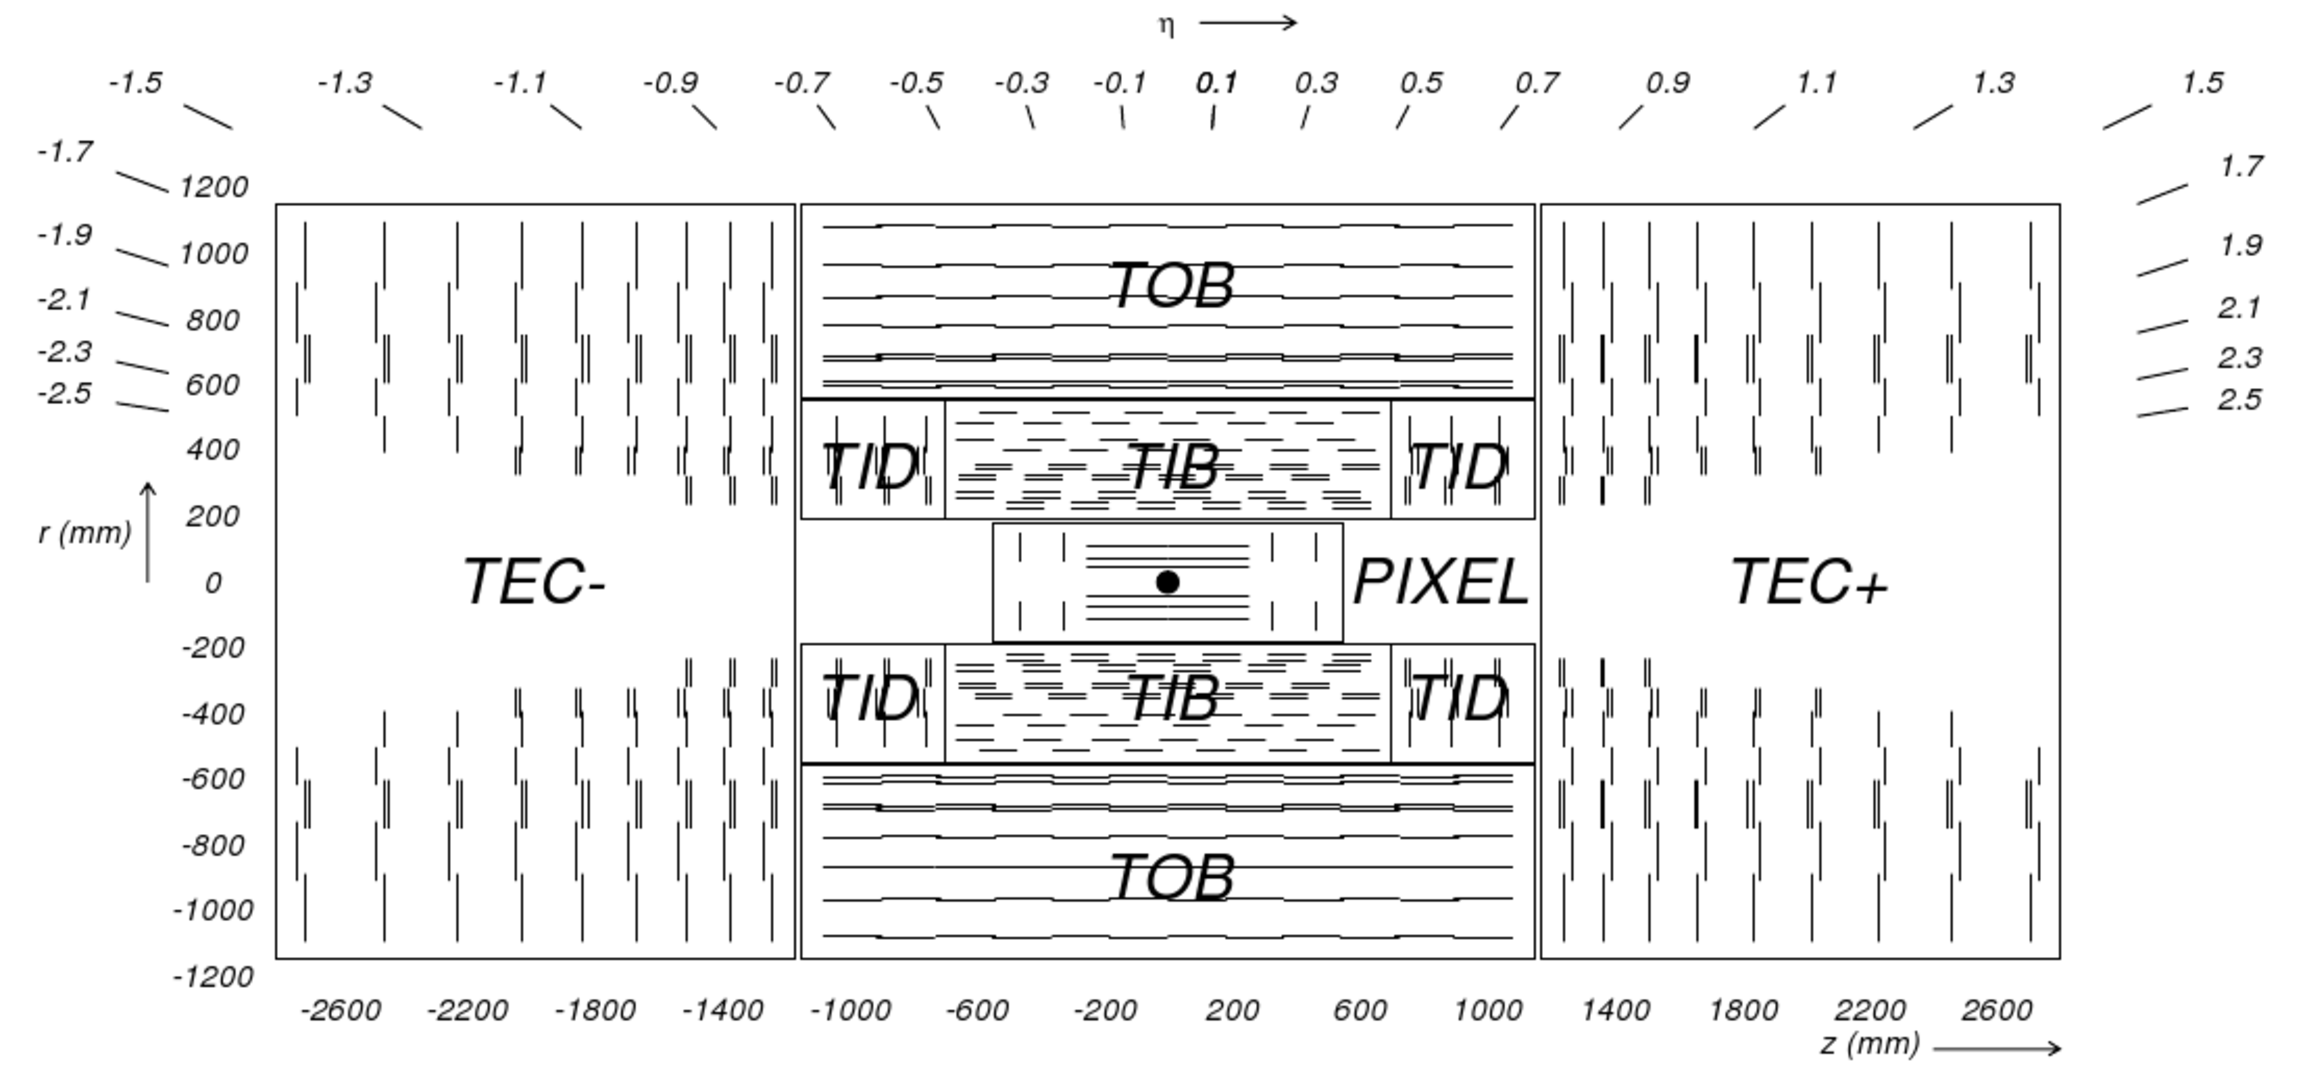
\includegraphics[width=0.6\textwidth]{ch3_figs/tracker_yz.pdf}
   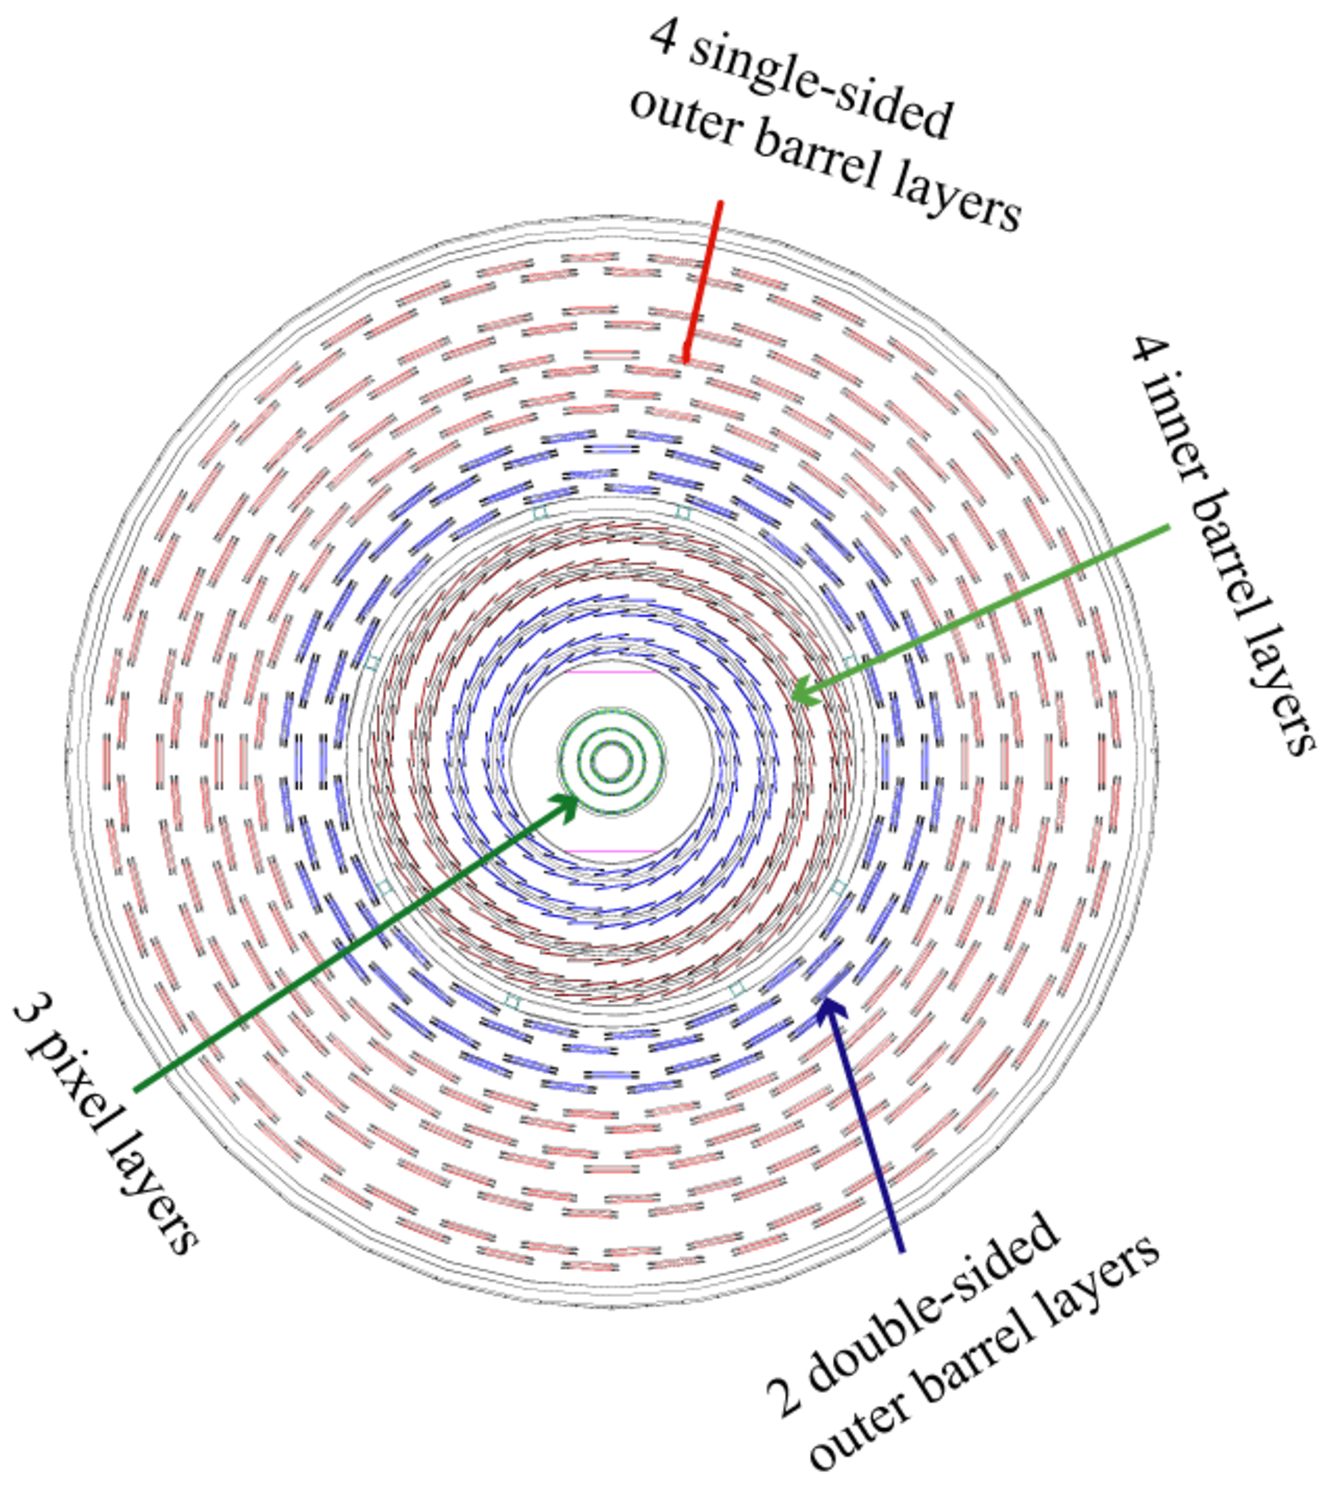
\includegraphics[width=0.25\textwidth]{ch3_figs/tracker_transverse_layers.pdf}
   \caption{The CMS silicon tracking system including both the pixel and strip detectors in y-z plane (left), and tranverse x-y plane (right).}
   \label{fig:cms_tracker}
 \end{center}
\end{figure}

\subsubsection{Strip Detector}
Outside the pixel detector is the silicon strip detector. Here, silicon strips are favored over pixels as they are less costly, and the resolution provided by the pixels
is not necessary at greater distances from the interaction point, allowing for larger and fewer silicon modules. 

The silicon strip detector consists of about 10 million strips in 10 layers, extending to 130 cm from the beam. 
The strip detector is comprised of 4 distinct sections of silicon strips, depicted in
Figure~\ref{fig:cms_tracker}. The outer most sections are the tracker outer barrel (TOB) and tracker end cap (TEC+,-) sections. 
Between the TOB and the pixels, sits the tracker
inner barrel (TIB) section, and the tracker inner endcaps (TID+,-).
The silicon strips in each section are different, specifically suited to that section.
Each silicon strip measures between 10-25 $\mu$m by 180 $\mu$m, depending on the position. The total detector area of the tracking system (pixels+strips) sums to more than
a tennis court of silicon. Precise tracking information is essential to measuring particle momenta and identifying particles in the strong magnetic field.

\subsection{ECAL}
The Electromagnetic Calorimeter (ECAL) measures the energy of particles that interact via the electromagnetic force. The ECAL is situated immediately outside the tracker
and is made of up thousands of lead tungstate ($PbWO_{4}$) crystals in three distinct sections. The ECAL provides good energy resolution, fast readouts, and radiation hardness
which make it ideal for recording the frequent events produced by the LHC. 

The ECAL is made up of three sections; the barrel, endcaps, and preshower, depicted in Figure~\ref{fig:cms_ecal}. The barrel section is cylindrical and covers the full $\phi$
range, and extends between $|\eta| < 1.479$ in y-z. The barrel consists of 61200 crystals, each measuring approximately 2.2 cm x 2.2cm x 23 cm. The length of each barrel
crystal translates to approximately 26 radiation lengths. The two endcaps sit on each end of the barrel, extending between $1.479 < |\eta|< 3.0$, 315 cm on either side of
the interaction point. There 14648 identical crystals in the endcaps, each measuring 3 cm x 3 cm x 22 cm. Like the crystals in the barrel, these crystals have a small taper
with the smaller face pointing towards the interaction point, mimicking the conical shapes of particle decay showers.
The preshower disc sits on the ends of the barrel and in front of the endcaps. The preshower measures 2.5 m in circumference and is 20 cm thick. The ECAL preshower consists of two layers
of lead, followed by silicon sensors measuring 2mm x 2mm. The preshower allows the ECAL to resolve nearby photon pairs, and discriminates against those coming from in-flight decays
of neutral pions. The scintillation light from each crystal is detected by Avalanche Photo Diodes (APDs) in the barrel, and a Vaccuum Photo Triodes (VPTs) in the endcaps.
These readouts convert the scintillation light to a voltage pulse that is passed futher downstream to the trigger and DAQ. 

After particles pass through the silicon tracking system, they enter ECAL. The ECAL measures the energy of electromagnetically-interacting particles from collisions, namely electrons and photons.
The choice of the lead tungstate material is motivated by needing to stop the particles, and also scintillate light effectively to allow an accurate energy measurement.
The stopping action is accomplished with the lead atoms in the crystal, while the scintillation is accomplished with
the crystalline oxygen. These combined properties produce photons (light) in proportion to the amount of energy deposited by the stopped particles.

\begin{figure}[hbtp]
 \begin{center}
   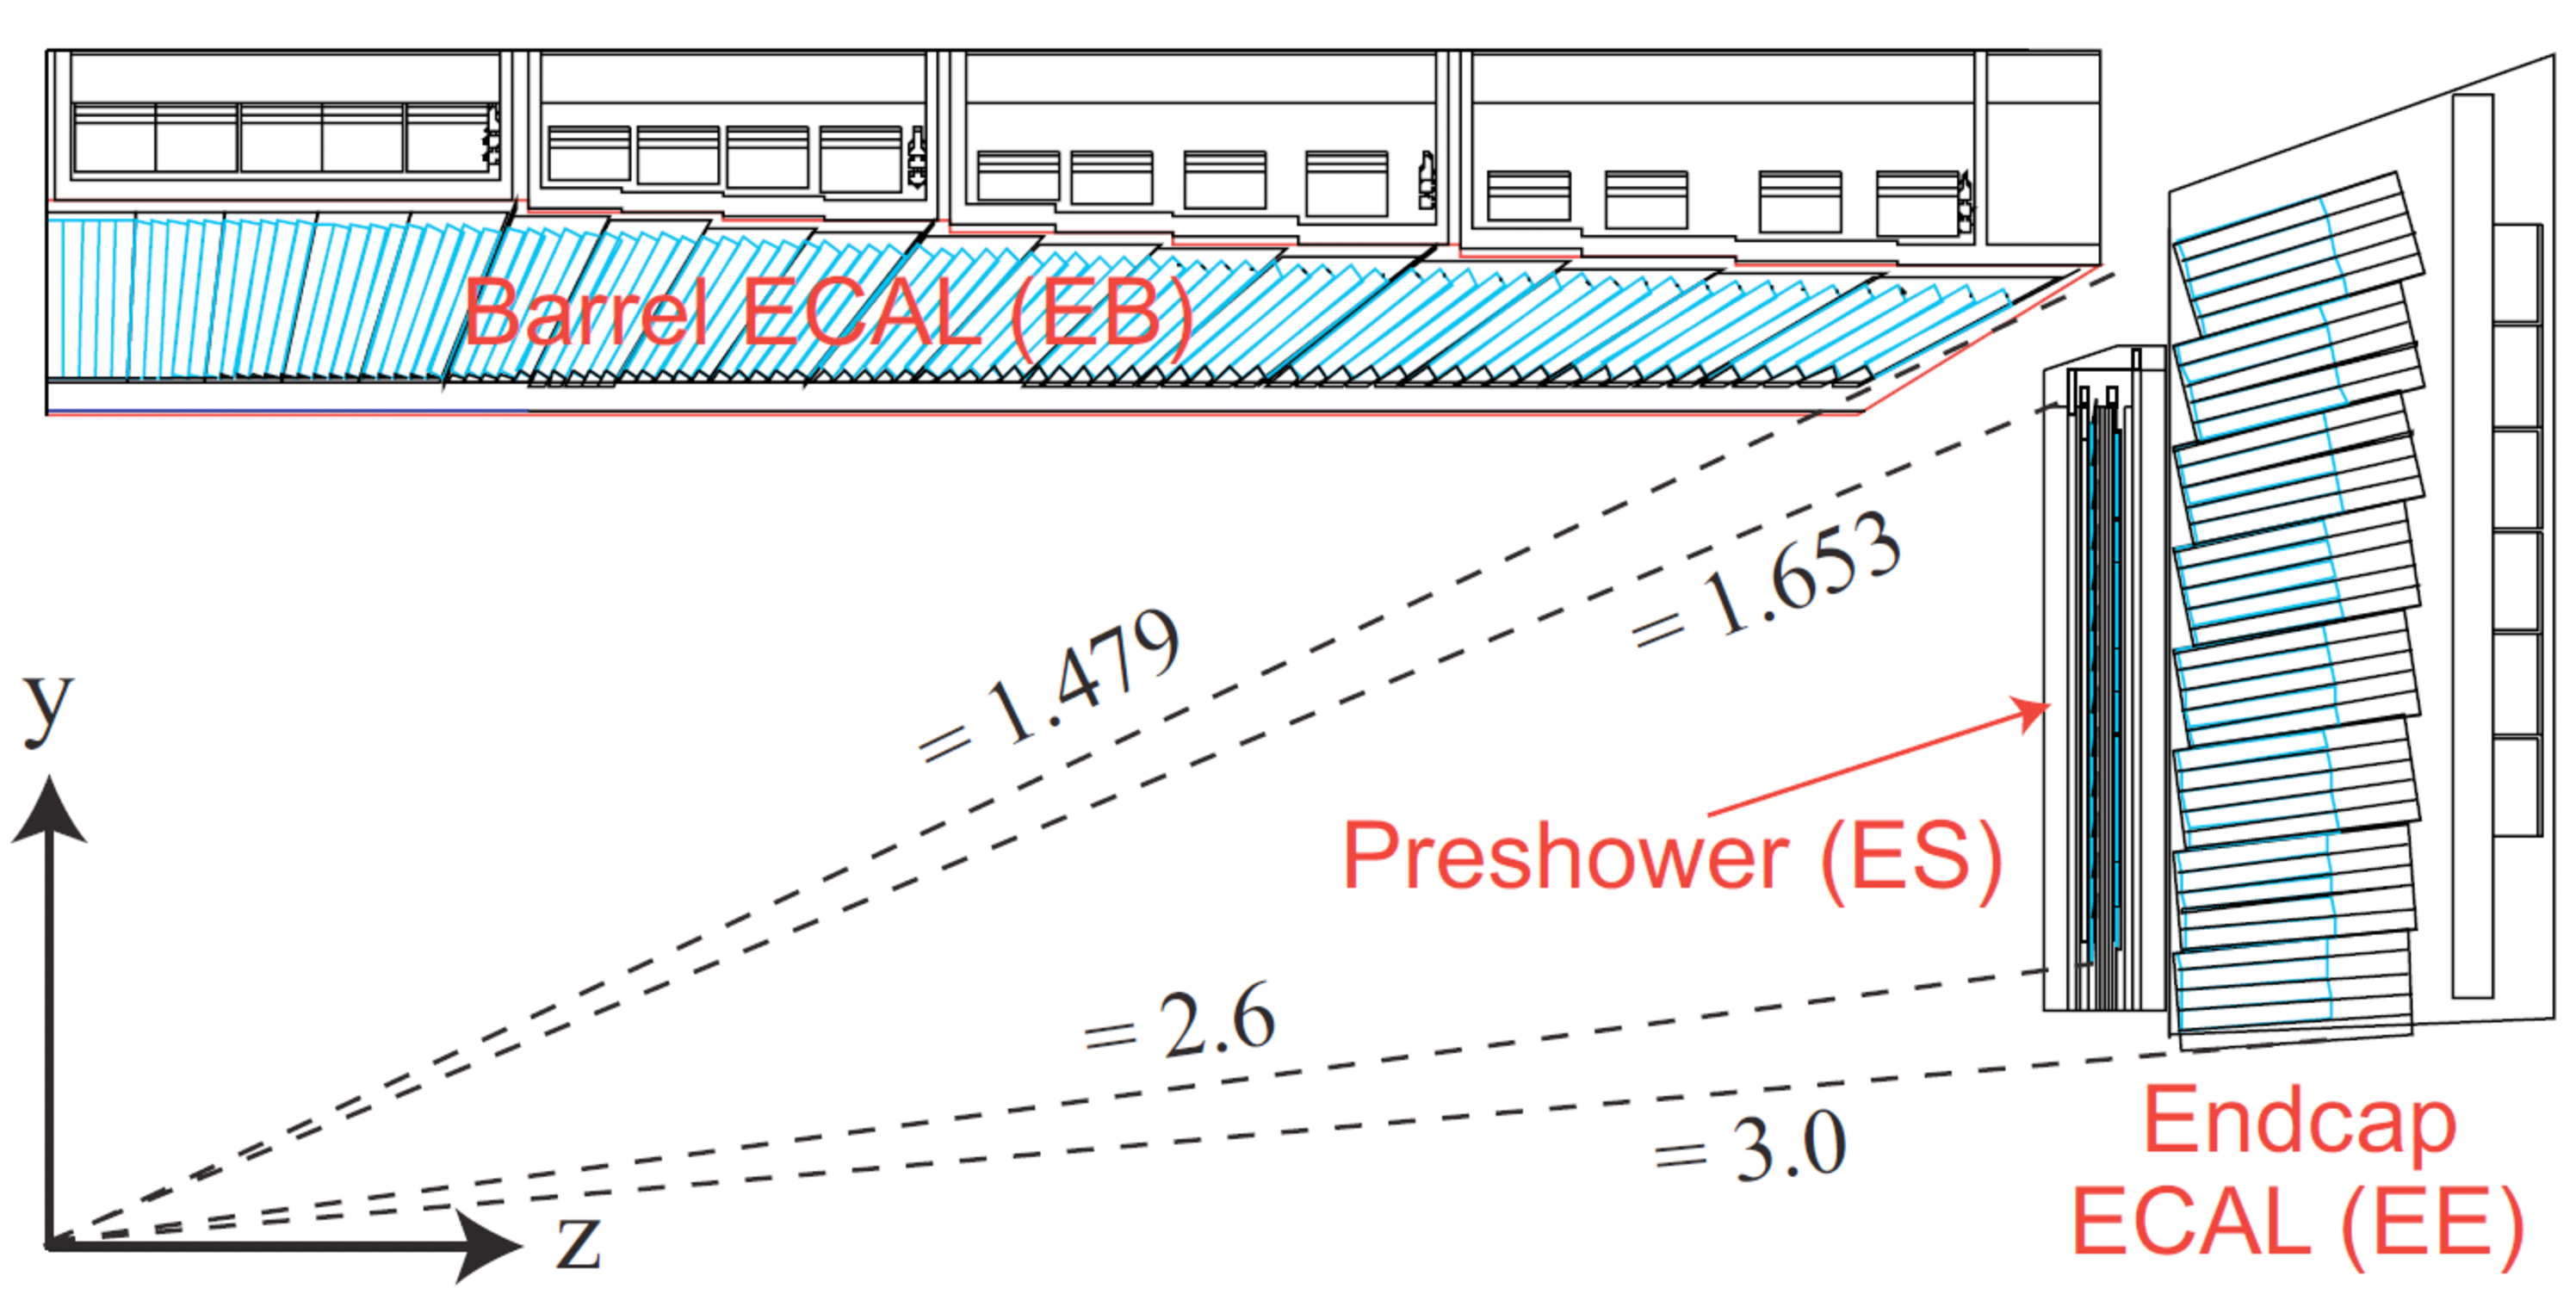
\includegraphics[width=0.9\textwidth]{ch3_figs/ecal_rapidity.pdf}
   \caption{Longitudinal view of one quarter of the ECAL.}
   \label{fig:cms_ecal}
 \end{center}
\end{figure}

\subsection{HCAL}
The CMS Hadronic Calorimeter measures the energy of hadronically-decaying particles and hadron jets which interact via the strong force. The HCAL sits outside and encloses the ECAL.
The HCAL is sampling calorimeter made up of alternating layers of brass absorber and plastic scintillator material in four separate sections. The HCAL provides energy resolution that helps reconstruct and tag hadronic
particle decays, as well as reconstructing the $missing transverse energy$ or \met, which can be interpreted as the presence of neutrinos. 

\begin{figure}[hbtp]
 \begin{center}
   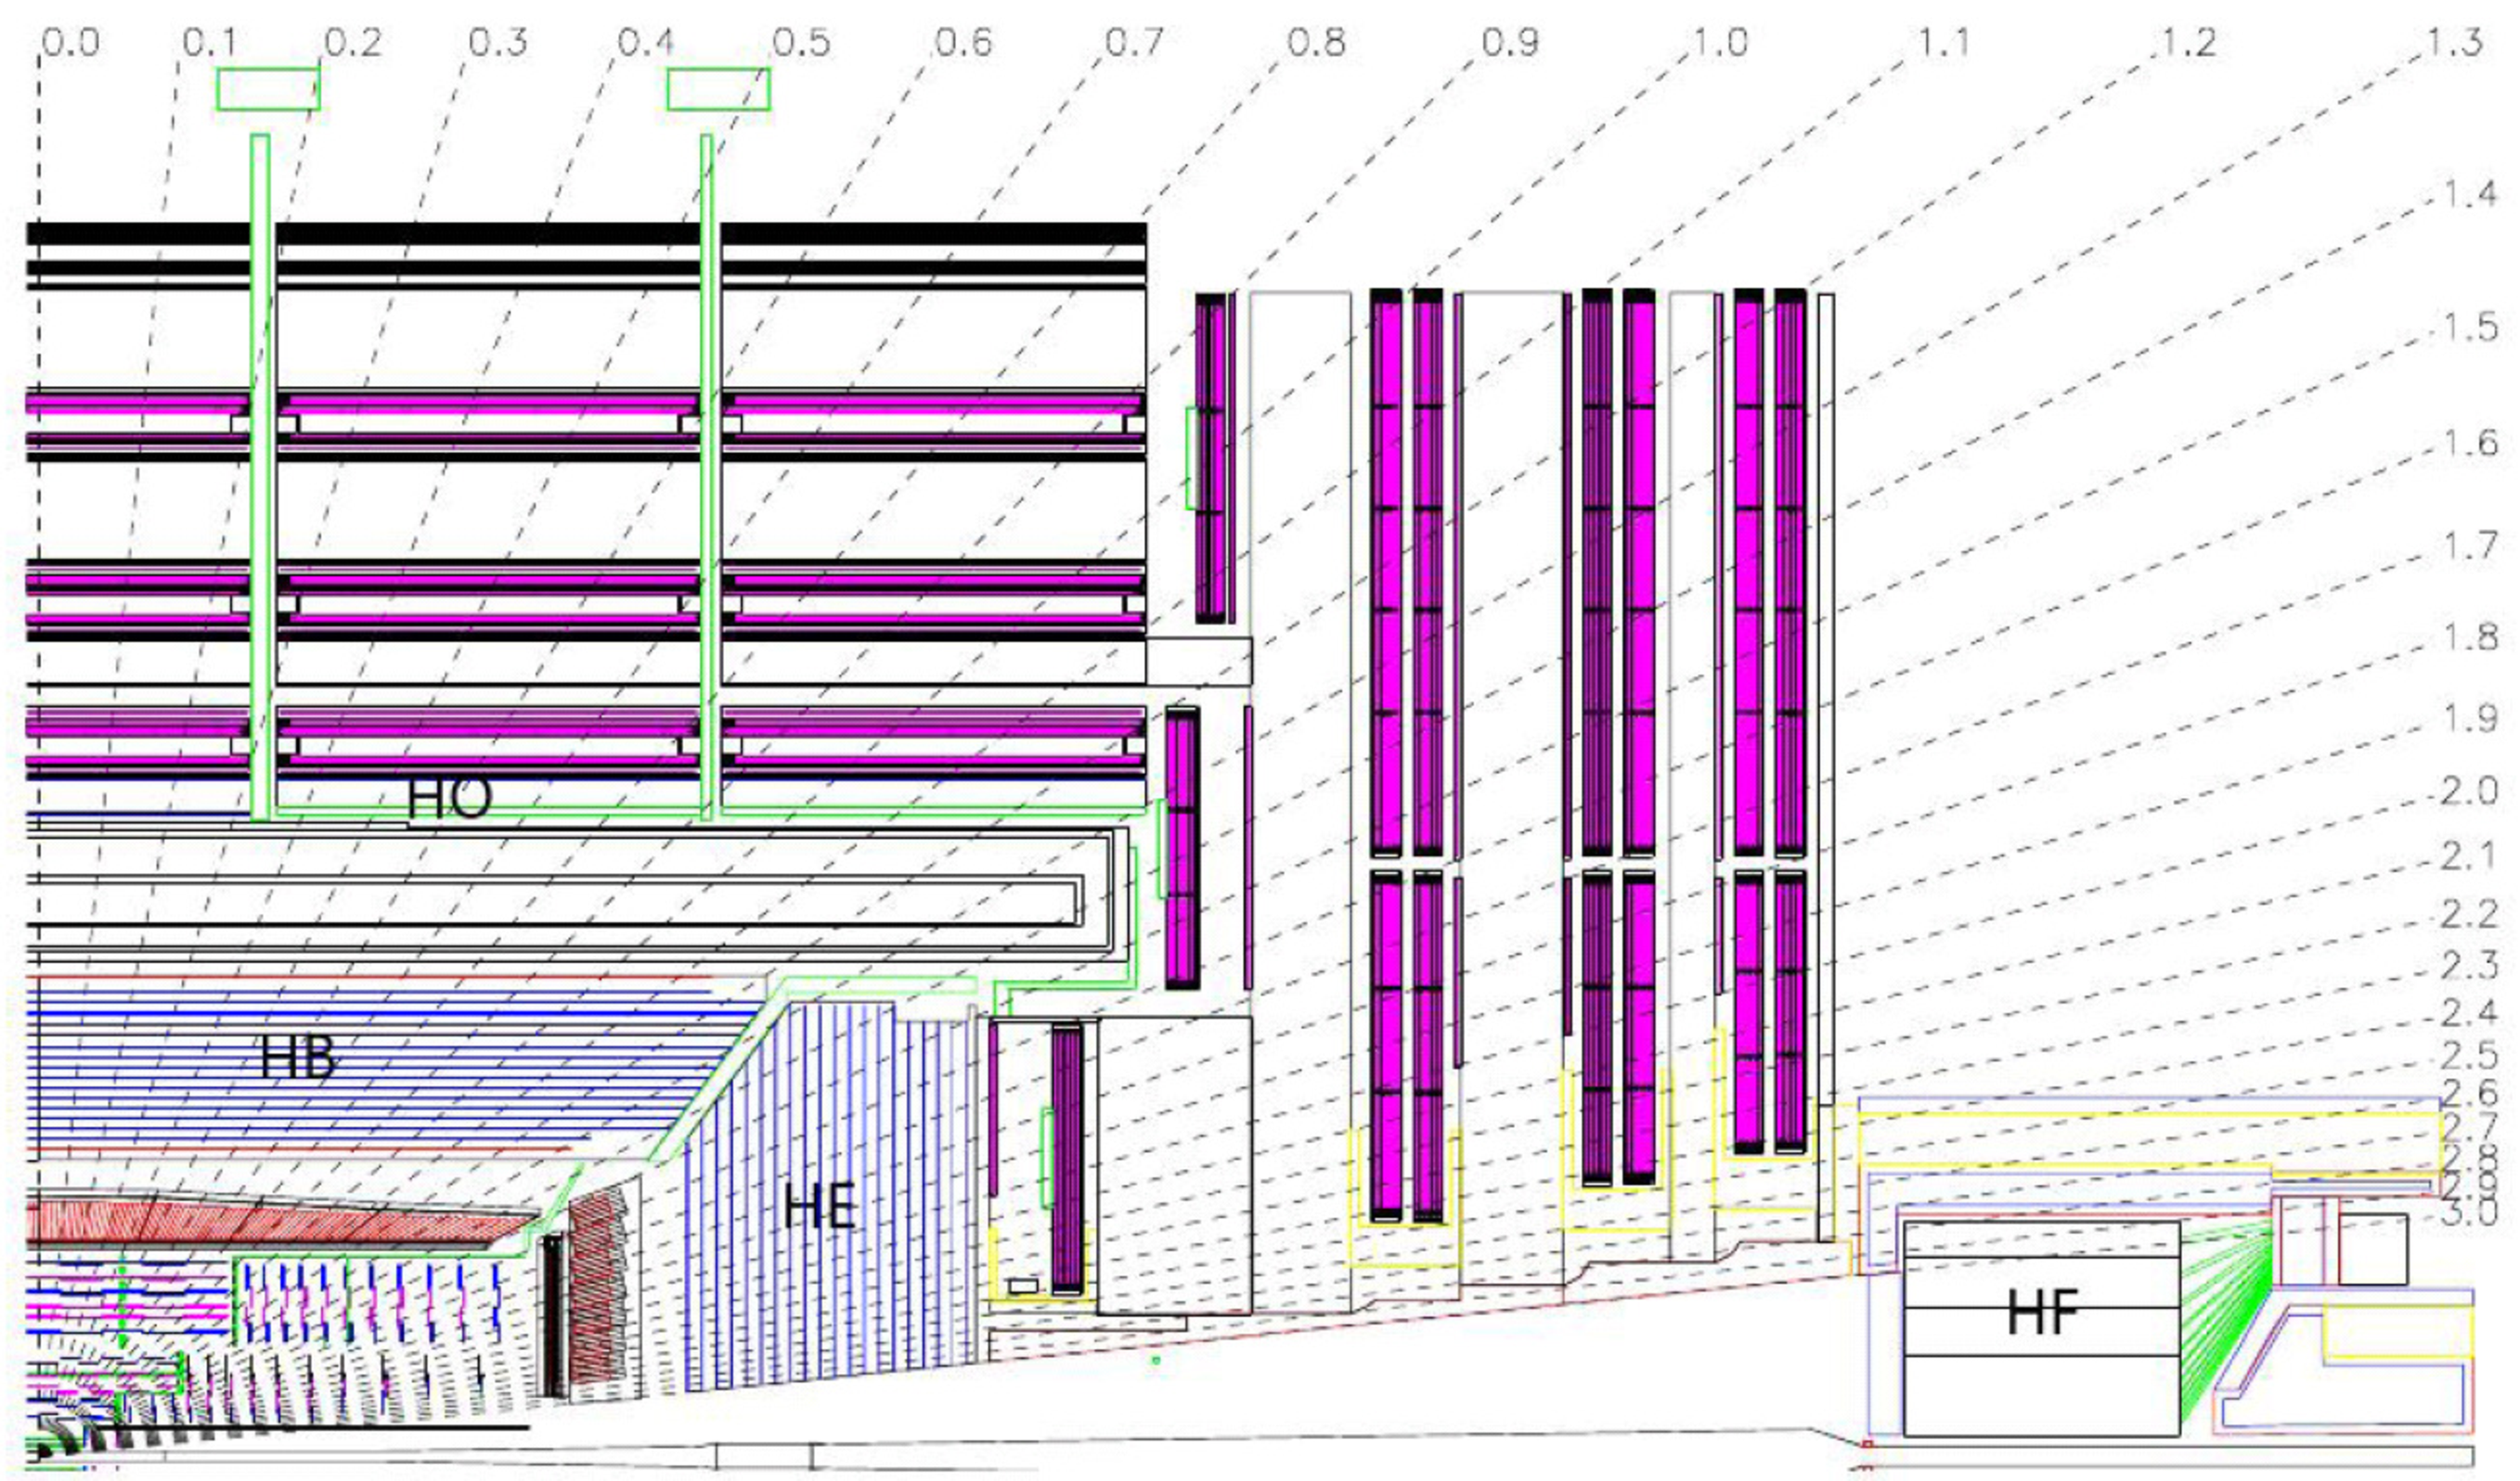
\includegraphics[width=0.9\textwidth]{ch3_figs/hcal.pdf}
   \caption{Longitudinal view of one quarter of the HCAL.}
   \label{fig:cms_hcal}
 \end{center}
\end{figure}

The four sections of the HCAL are the barrel (HB), the endcaps (HE), the outter barrel (HO) and the forward HCAL (HF) in Figure~\ref{fig:cms_hcal}. The barrel extends from 1.77 m to 2.95 m from the interaction point and
sits between the outside of the ECAL barrel and the inside of the magnet coil in the transverse plane. The HB covers a psuedorapidity range of $|\eta| < 1.3$.
The endcaps cover a psuedorapidity of $1.3 < |\eta| < 3$, which contains approximately 34$\%$ of final state particles. The HO sits outside and around the solenoid coil covering the same psuedorapidity range
as the HB. The HO utilizes the magnet coil as an additional absorbing layer ensuring detection of any particle exiting the HB. The HF sits outside of all other subdetectors at $\pm$11 m from the interaction point in the z-direction,
covering a psuedorapidity range of $3.0 < |\eta| < 5.0$. The HF was specially designed to resist the intense radiation deposited in this forward region. Within each plastic scintillator tile are optical wavelength-shifting fibers.
Measuring less than 1 mm in diameter, these fibers connect to other optical fibers which send the light signals to Hybrid Photodiodes (HPDs) for readout. The fast and radiation-resistant HPDs amplify the light and convert it
into an electronic signal via the photoelectric effect.

As strongly-interacting particles travel through the HCAL, they interact with the dense brass absorber material decaying and producing showers of secondary particles which further cascade and travel through the scintillator and absorber material.
As the shower particles pass through the scintillator material, they emit a blue-violet light. This blue-violet light is then converted to green light via the wavelength shifting fibers and send to the HPDs for readout. Like the ECAL,
the amount of light emitted corresponds to the amount of energy deposited. 

\subsection{Solenoid}
Central to the design and name of CMS, the CMS magnet is the largest superconducting solenoid of its kind in the world.
At 12 m in length, it produces a field of nearly 3.8 T inside the 6 m diameter free bore, with the flux returned through a 10000 ton iron yoke.
The magnetic field outside the free bore in the muon chambers is approximately 2 T.  
Similar to the LHC magnets, the solenoid uses NbTi coils cooled to 1.8 K but carries a current of over 19000 amps. When fully energized, the magnet
stores 2.6 GJ of energy, enough to power 24 American homes for 1 day\cite{magnet_energy}. The central barrel of the solenoid sits between the HCAL and the muon chambers, with the return yoke iterwoven with the muon chambers.

A strong magnetic field is essential for measuring the momentum of charged particles. Charged particles moving in a magnetic field are subject to the Lorentz force, described in
equation~\ref{eqn:lorentz_force} 

\begin{equation}
\label{eqn:lorentz_force}
 \vec{F} = q\vec{v} \times \vec{B}
\end{equation}

The particles from hard inelastic collisions typically have a large momentum component in the transverse plane, since the momentum of the opposing beams before the collision in the z-direction cancel each other.
The solenoid produces a magnetic field along the z-direction and by the right-hand-rule from the cross product in equation~\ref{eqn:lorentz_force}, this means the particles experience a centripetal force, which
curves or deflects their trajectories. By setting the Lorentz force equal to the centripetal force in equation~\ref{eqn:lorentz_qvb}, the momentum and charge of the particle can be found by measuring the radius of the track. 
Thus the field produced by the CMS solenoid together with accuarate track reconstruction, allows for precise momentum measurements of the particles.

\begin{equation}
\label{eqn:lorentz_qvb}
 qvB = \frac{mv^{2}}{r}
\end{equation}

\subsection{Muon Chambers}
Central to both the name and function of CMS, the muon chambers are solely dedicated to detecting and measuring muons.
Because muons are so heavy, they are not stopped by any other part of CMS and thus are the only particle to pass through all other CMS subdetectors.
The muon chambers are the outermost subdetector for this reason. The muon chambers are comprised of 3 unique gas detection systems consisting of Drift Tubes (DTs),
Cathode Strip Chambers (CSCs), and Resistive Plate Chambers (RPCs), which each serve a specific purpose. Each of the gas chambers produce voltage pulses as muons pass through and leave hits.
Similar to the tracker, the hits are reconstructed into muon tracks, which can then be used to determine the precise momentum of the muon in the magnetic field.  

\begin{figure}[hbtp]
 \begin{center}
   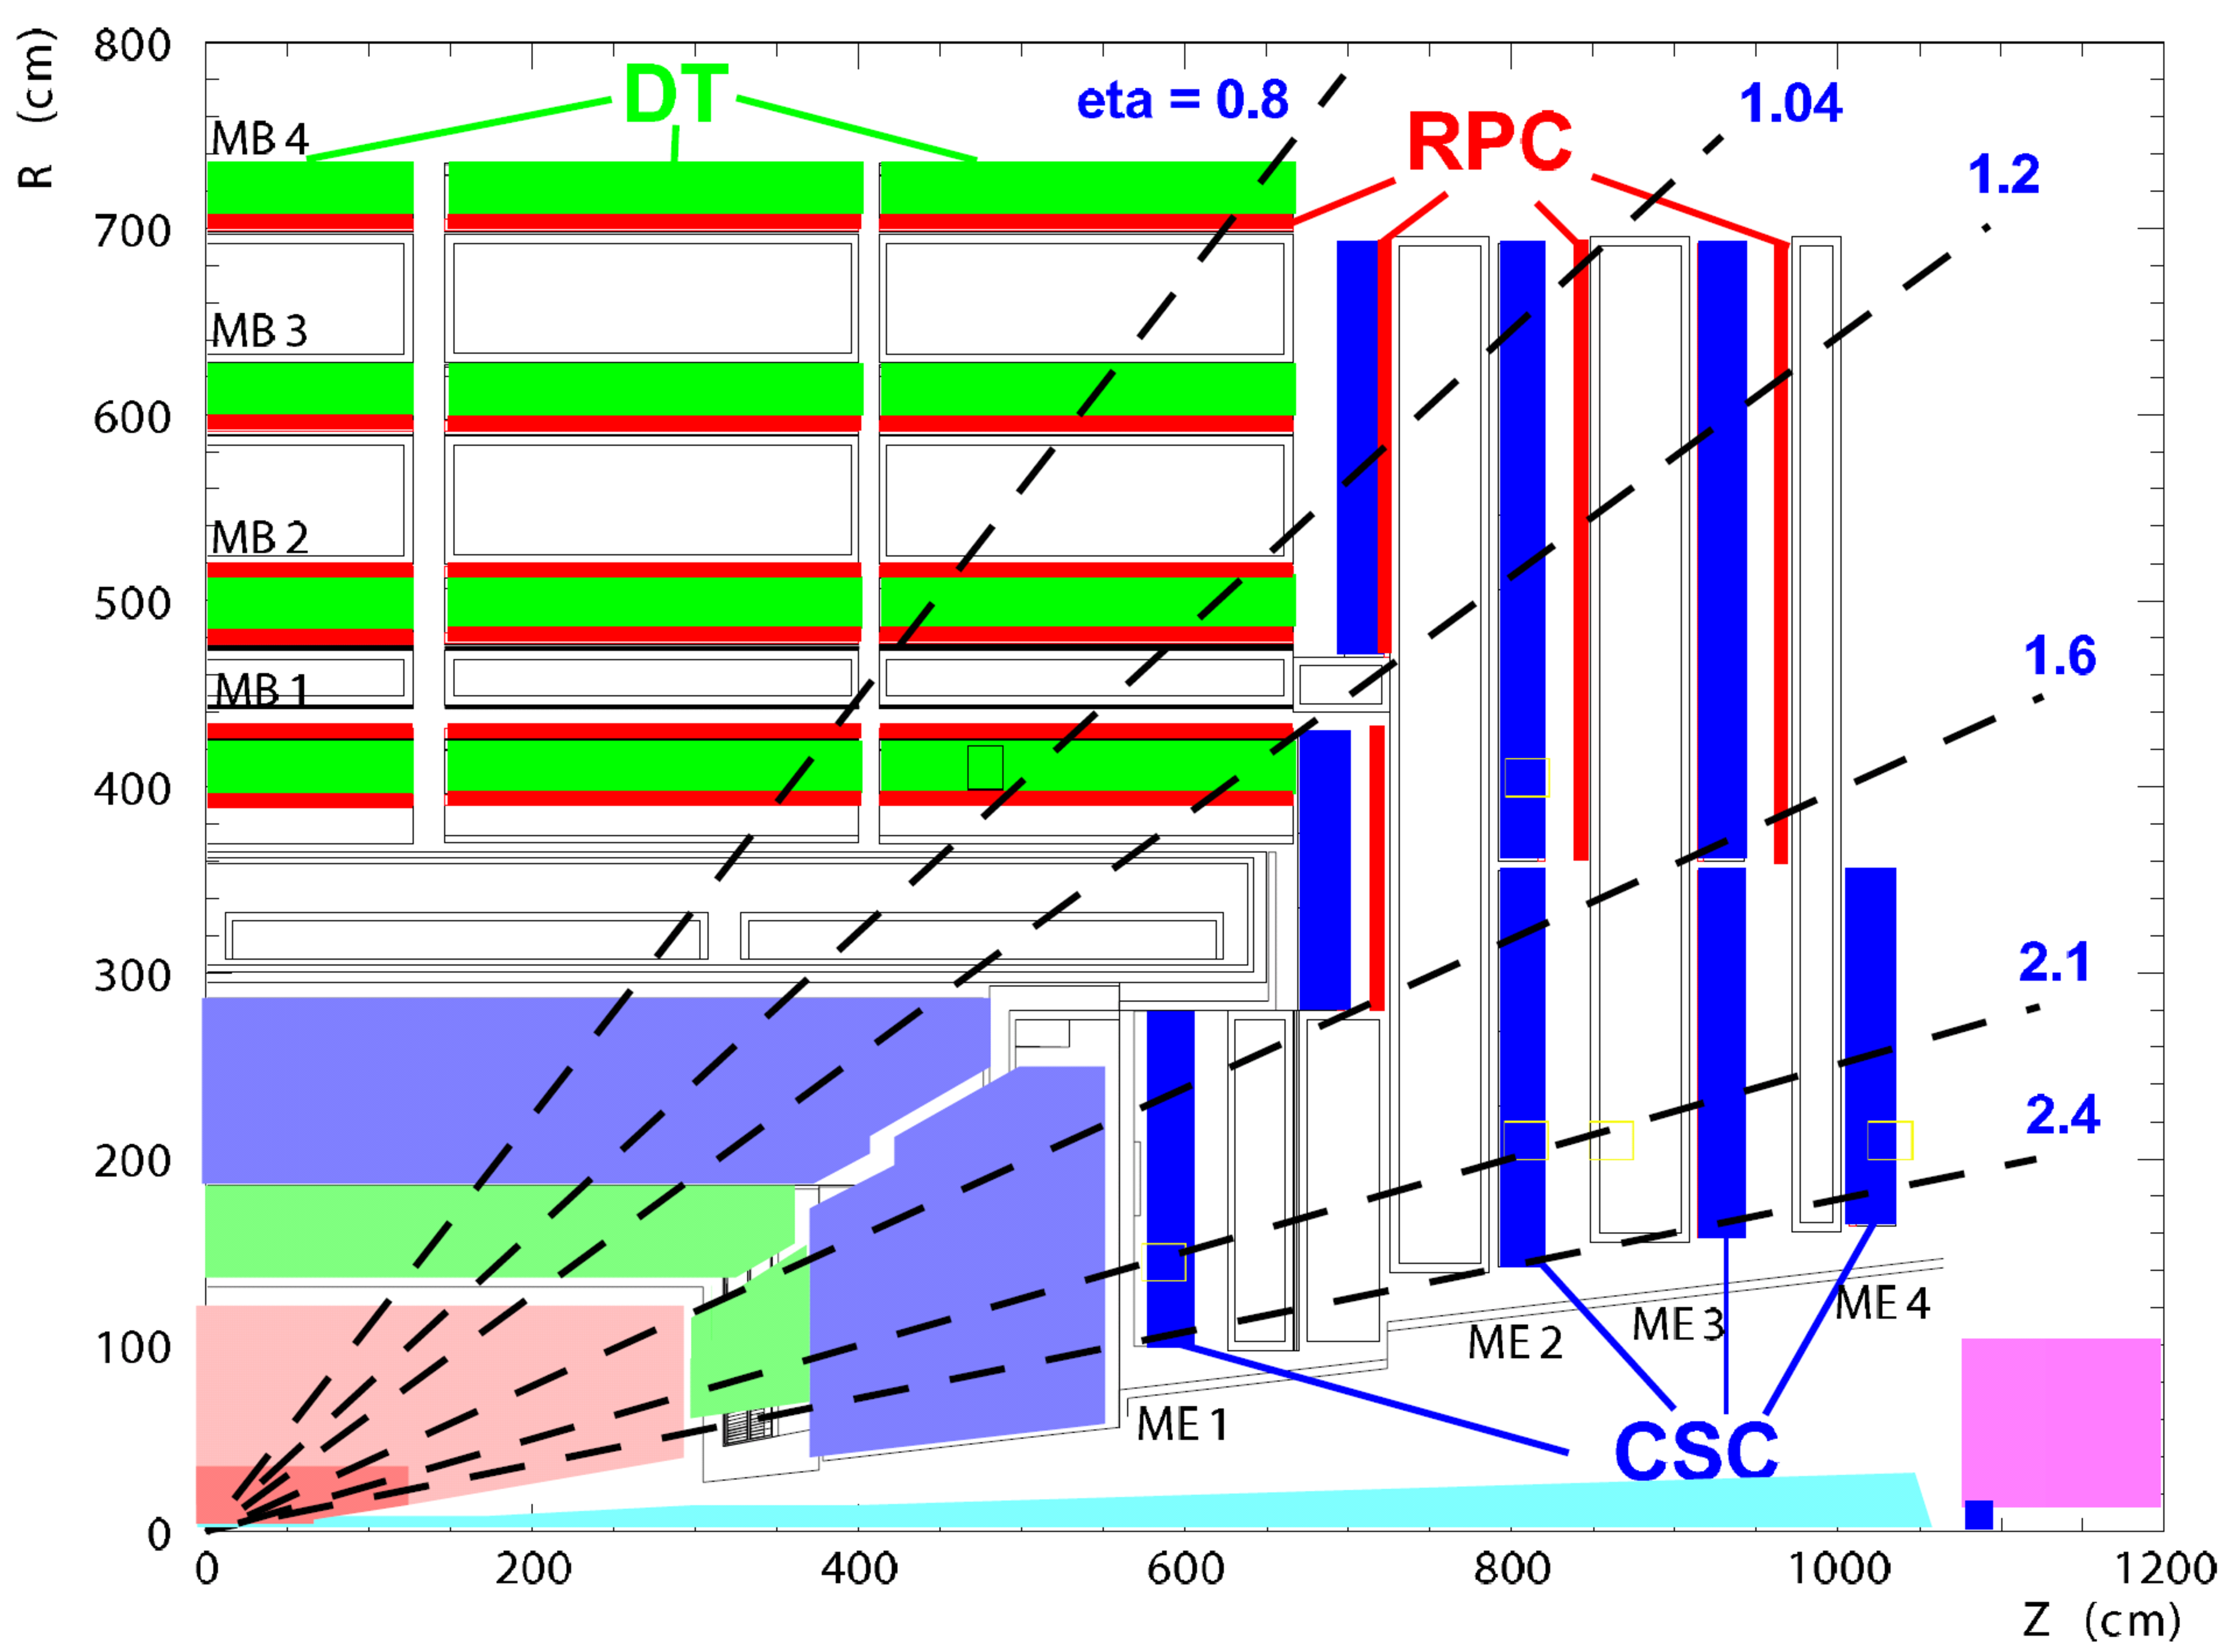
\includegraphics[width=0.9\textwidth]{ch3_figs/cms_muonchamber.pdf}
   \caption{Longitudinal view of one quarter of the CMS muon chambers.}
   \label{fig:cms_muonchamber}
 \end{center}
\end{figure}

The DTs cover the barrel region of the detector. There are three concentric cylindrical layers each containing 60 drift tube chambers and one additional outer layer with 70.
Each drift tube measures 4 cm wide and is filled with a mixture of 85$\%$ Ar and 15$\%$ $CO_{2}$ gas. A 2.4 m long positively-charged current-carrying wire in the center of the drift tube attracts electrons
from the ionization of the gas caused by a passing muon. The drift tubes provide two coordinates for the muon position by measuring where along the wire the
electrons hit, and the time it takes to register, since the speed of the electrons in the gas is constant. The DTs are used in the barrel only, where there are lower particle fluxes
and intensities. 

\begin{figure}[hbtp]
 \begin{center}
   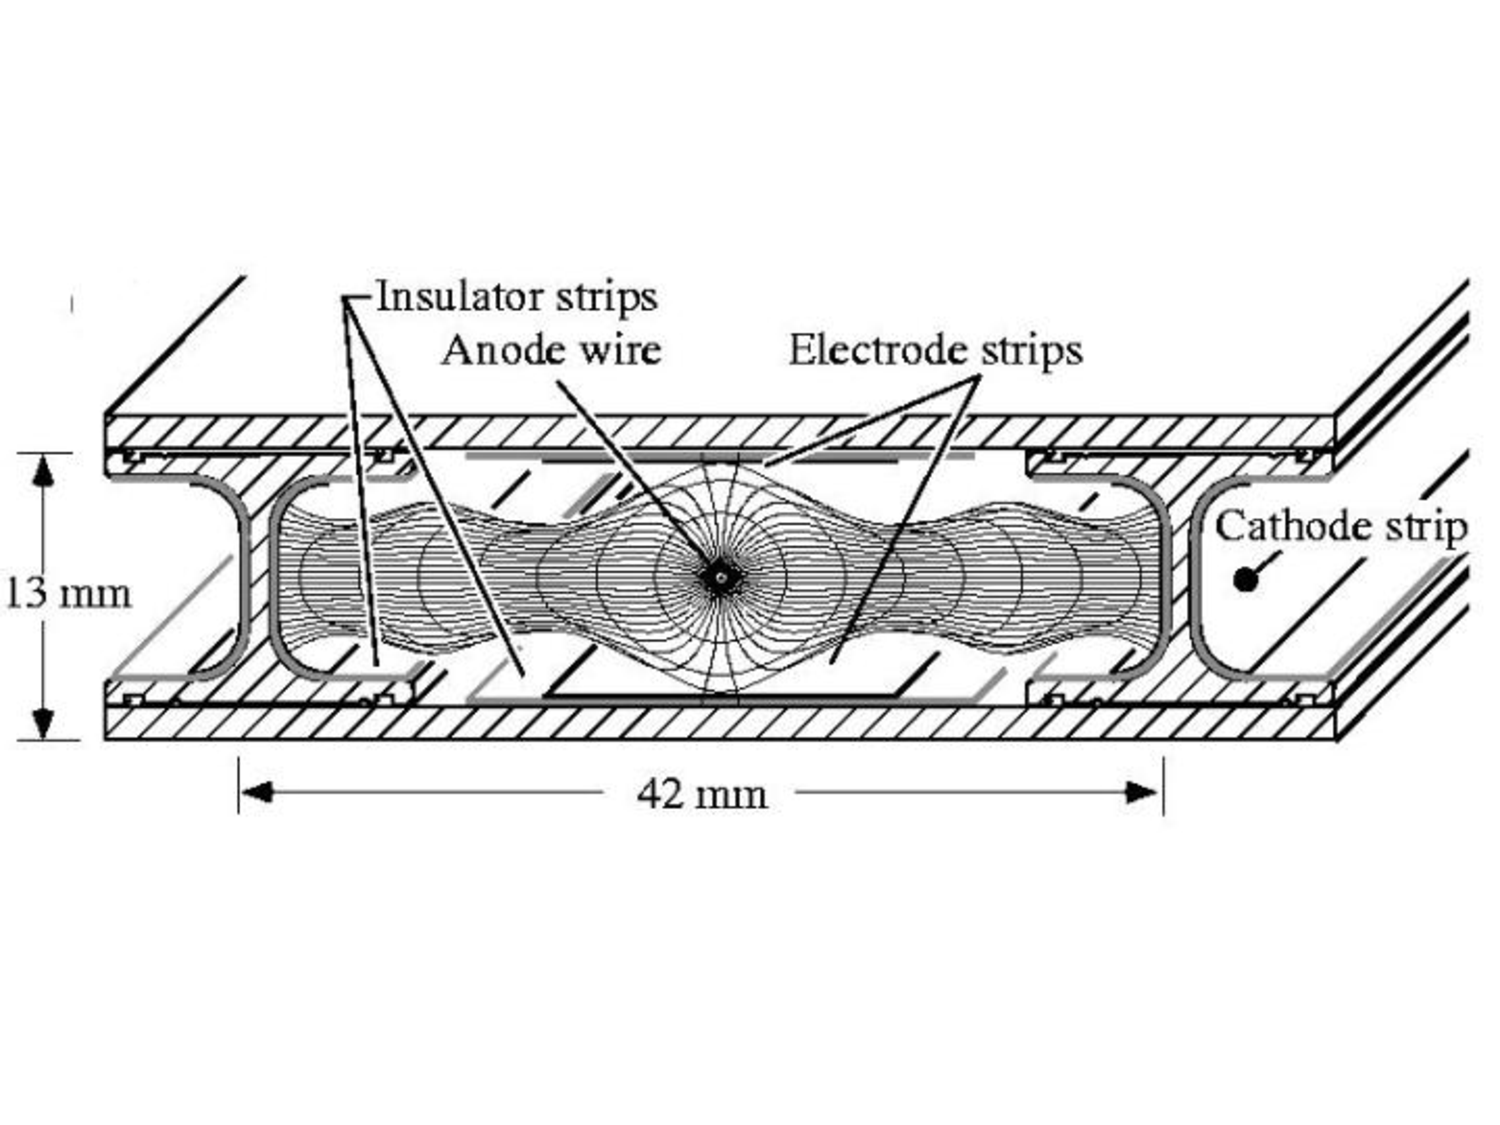
\includegraphics[width=0.9\textwidth]{ch3_figs/cms_dt.pdf}
   \caption{A map of the electric field of the drift tubes in absence of magnetic field. In the presence of a magnetic field there is a small distortion that is accounted for.}
   \label{fig:cms_dt}
 \end{center}
\end{figure}

The CSCs are used only in the endcaps, where there is a greater particle intensity and an uneven magnetic field. 468 CSCs in 7 layers make are in the endcaps, where each chamber is trapezoidal in shape.
Each chamber consists of positvely charged anode wires which cross negatively charged cathode strips that are enclosed in a chamber filled with gas. As muons enter a
CSC, they ionize the gas causing freed electrons to travel to the positive wires and positive charges migrate towards the cathode strips. The charge pulses are detected in both the strips
and the wires, which are perpendicular to each other, providing two coordinates for each muon hit. The CSCs provide good position information quickly, making them suitable for use in the endcaps. 

\begin{figure}[hbtp]
 \begin{center}
   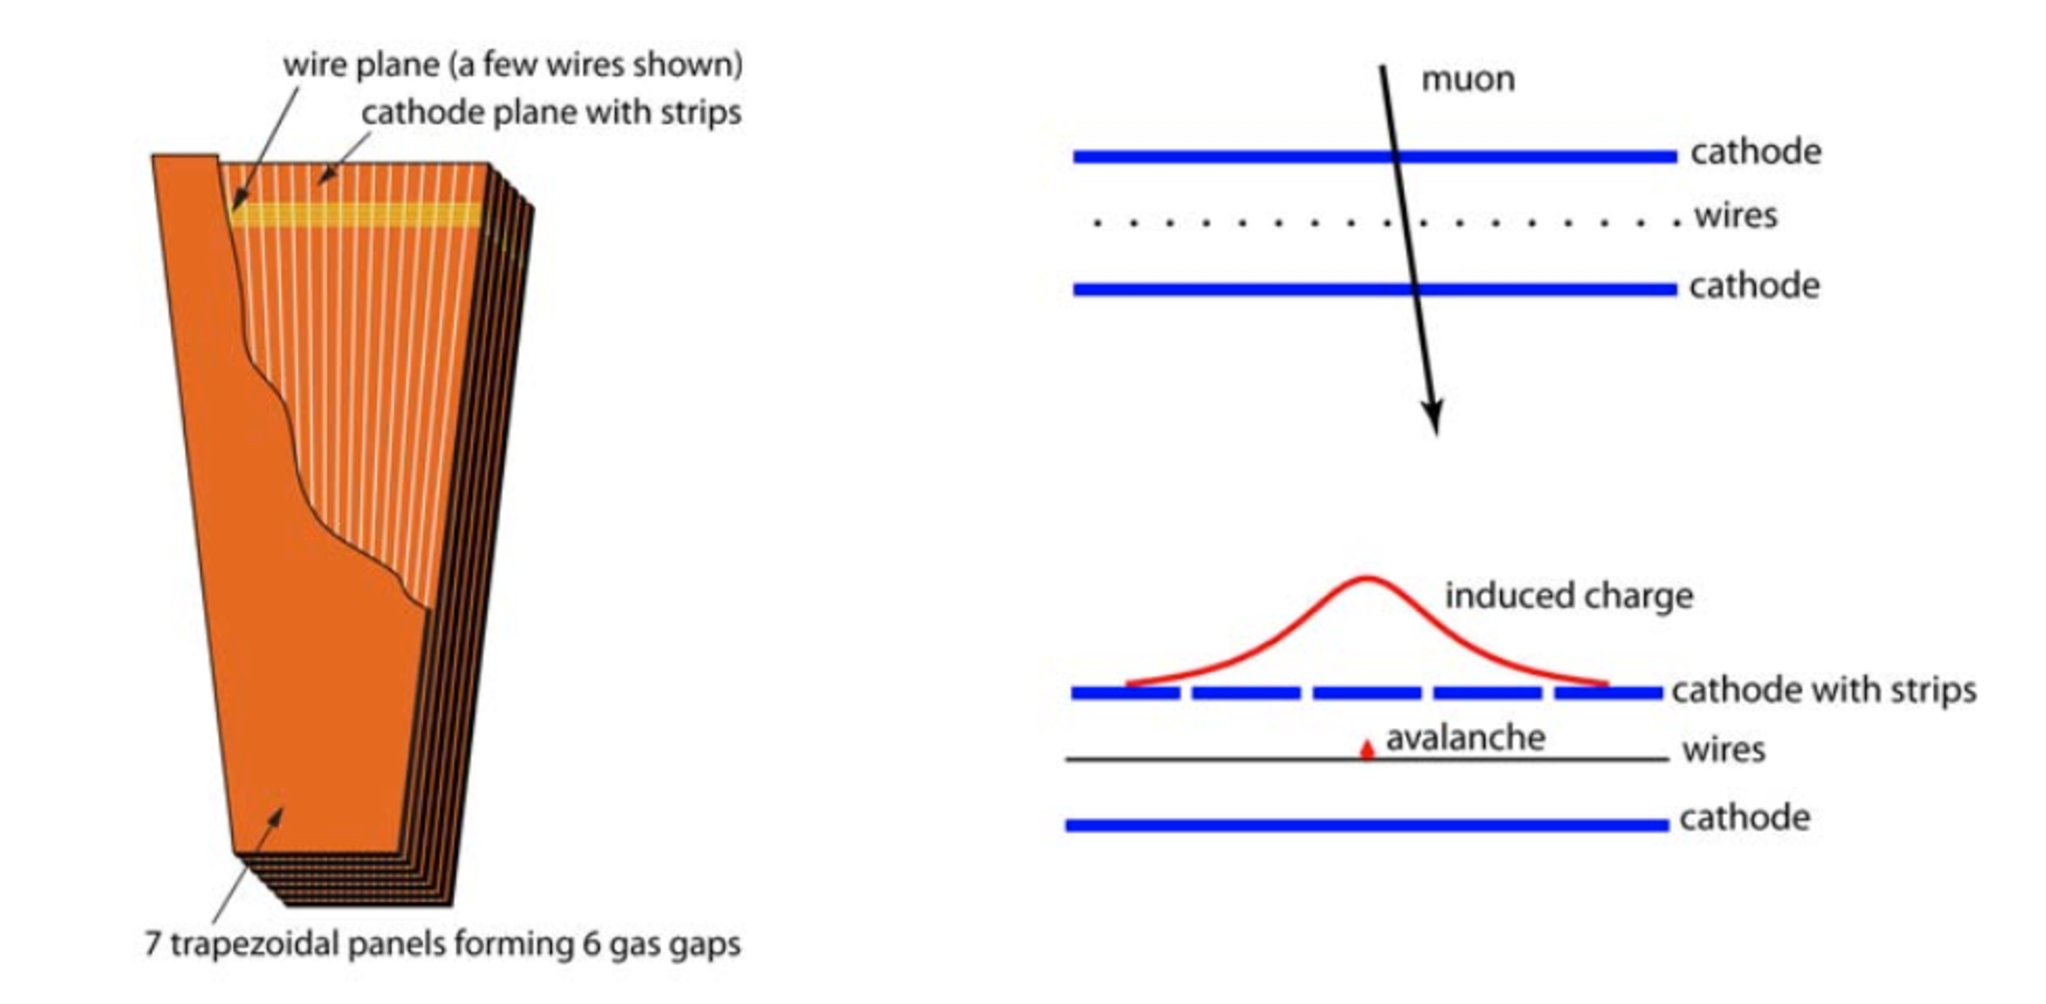
\includegraphics[width=0.9\textwidth]{ch3_figs/cms_csc.pdf}
   \caption{CSC module (left) and a depiction of the CSC opteration (right). The strips provide preices position information.}
   \label{fig:cms_csc}
 \end{center}
\end{figure}

The third type of muon detector used is the RPC. Unlike the DTs and the CSCs, the RPCs are used in both the barrel and the endcaps. The RPCs are characterized by their fast response time, which makes thenm suitable for triggering.
Thanks to this very fast response of < 1 ns, the RPCs can easily identify which bunch crossing a given muon is associated with, since the bunch time spacing is 25ns.  
Each RPC consists of two oppositely-charged parallel plates within a gas volume and detecting strips of electrodes. These detecting strips quickly reconstruct muon tracks allowing for fast triggering decisions based on muon momentum.  

\begin{figure}[hbtp]
 \begin{center}
   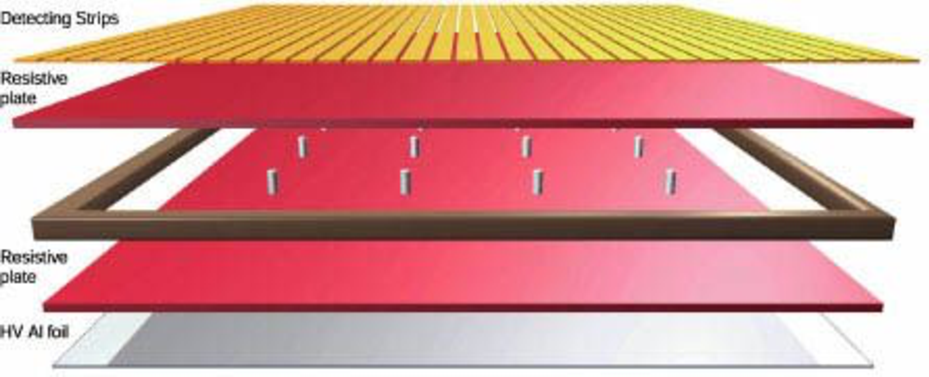
\includegraphics[width=0.9\textwidth]{ch3_figs/cms_rpc.pdf}
   \caption{A qualitative depiction of an RPC.}
   \label{fig:cms_rpc}
 \end{center}
\end{figure}
 
\subsection{Trigger and Data Acquisition}

The LHC collides proton bunches at a frequency of 40 MHz, making high event rates, and efficient data collection and filtering necessary. This task is accomplished with the trigger and Data Acquisition system (DAQ). Because not all collisions can be recorded,
and most collisons don't produce events that warrant further analysis, the trigger ``fires'' on interesting events only, and sends the information readout in each subdetector to the DAQ. The CMS trigger is comprised of two parts or levels.
The Level 1 (L1) is the frontline of the CMS trigger system, comprised of firmware and basic software that is directly connected to each subdetector's readout electronics. The second part of the trigger is called the High Level Trigger (HLT)
and is entirely software-based, running a filter farm of high-performance CPUs. 

The L1 is the first place where an event can be discarded or selected based on predefined conditions. From an event rate of 40 MHz produced by the LHC, the L1 filters and reduces this to between 80-100 kHz.  
Each subdetector readout, with the exception of the silicon trackers, is directly connected to the L1. Since the trackers have very high occupancies, and millions
of pixels and strips, sophisticated track reconstruction takes much longer than is acceptable for a L1 trigger decision. Therefore when the L1 fires based on other subdetector information, the tracker is immediately readout and the information is saved
but not reconstructed. The software portion of the L1 consists of 128 algorithms called triggers or bits, that are constantly processing detector readout information. Any one trigger accepting an event, will pass all the detector information downstream
to the HLT. 

The HLT receives events that pass the L1, and is the final filter that determines which events are saved or discarded. This means that all events passing the HLT are saved and reconstructed for later analysis.
The HLT reduces the L1 input rate from 100 kHz to around 1 kHz. The HLT software is the foundation on which the rest of the offline CMS analysis is built. The HLT software consists of over 400 trigger algorithms that make accept/reject decisions
based on quantities such as particle momenta, multiplicity, energy, position, and other more sophisticated variables that are available thanks to the advanced event reconstruction that takes place at the HLT.
The more than 400 HLT algorithms are gouped into categories based on the specific types of objects that fire the trigger such as electron/photons, muons, Jets/MET etc. These groups are called primary datasets and only events which passed a trigger
allocated to that primary dataset will be found in the associated dataset. Common examples of primary datasets include SingleEG, DoubleEG, SingleMu, DoubleMu, MuonEG etc. The events are then sent further downstream grouped together in these primary datasets.
The HLT and L1 algorithms are thoroughly tested and highly efficient at passing the objects they are
designed to accept. Typical HLT trigger efficiencies are well above 90$\%$. See the muon efficiency at the HLT in Figure~\ref{fig:hlt_eff_muons} below. 

\begin{figure}[hbtp]
 \begin{center}
   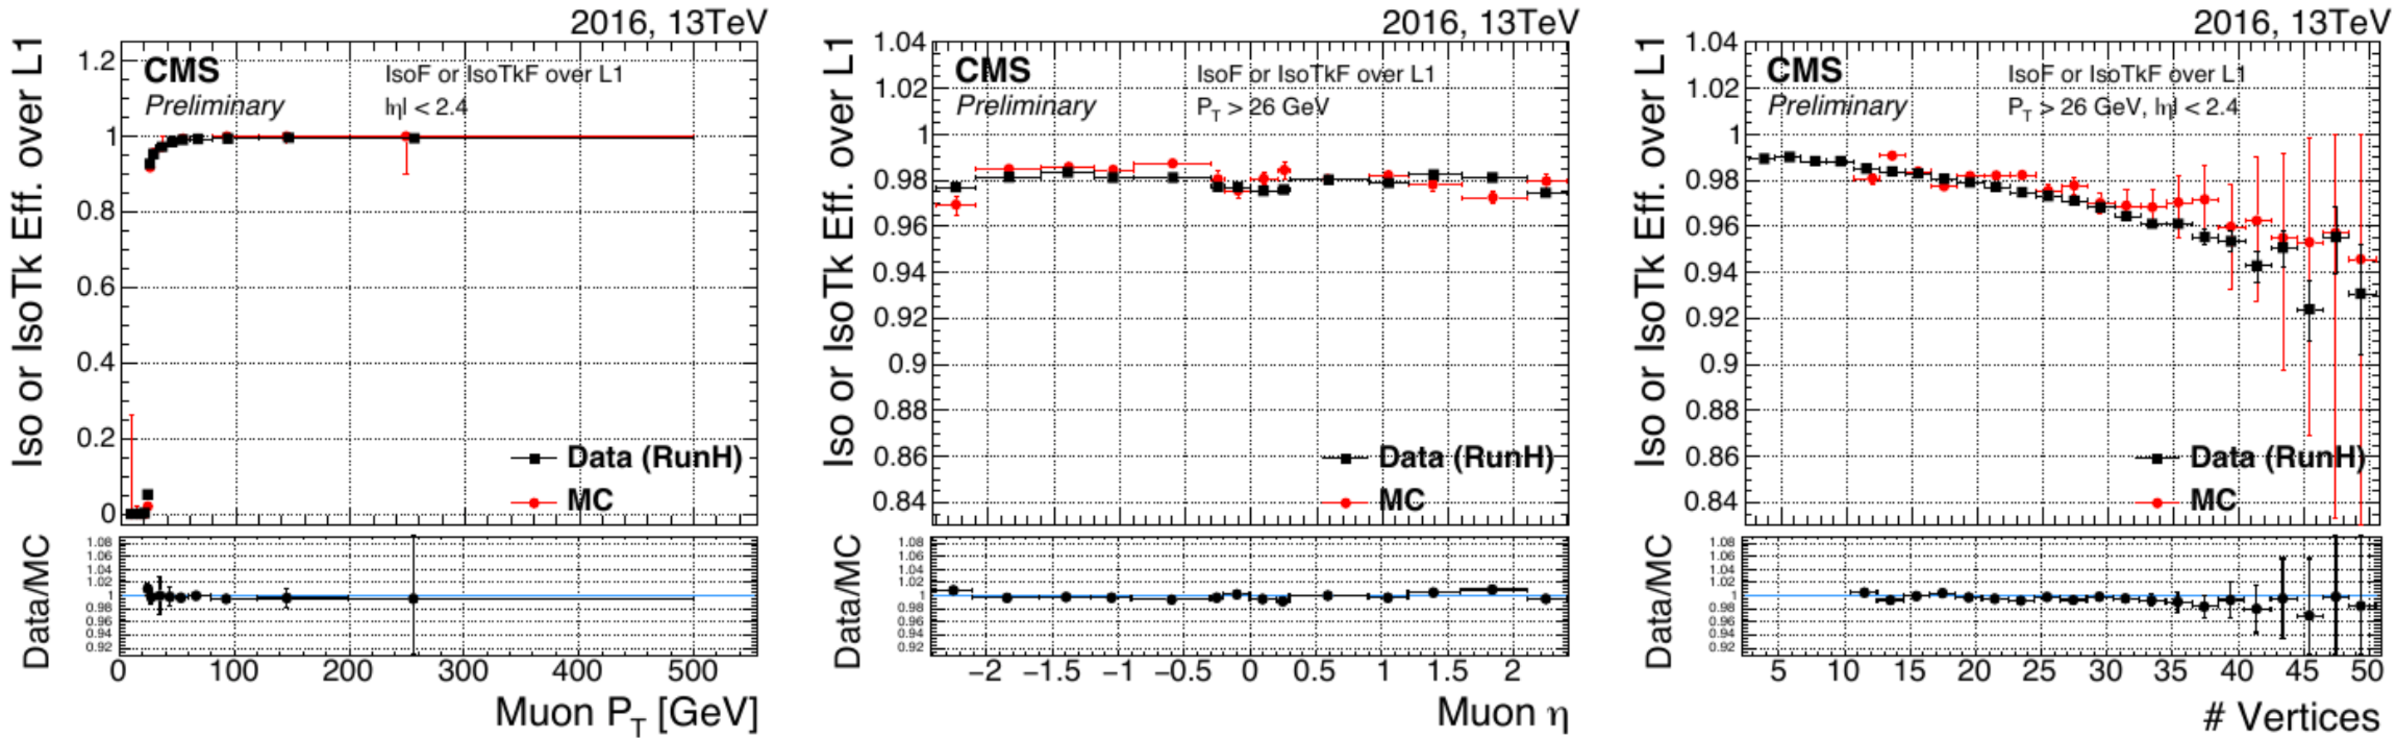
\includegraphics[width=0.9\textwidth]{ch3_figs/hlt_eff_muons.pdf}
   \caption{Muon trigger efficiency at the HLT as a function of muon transverse momenta, psuedorapidity, and number of reconstructed vertices.}
   \label{fig:hlt_eff_muons}
   %%https://indico.cern.ch/event/512834/contributions/2349020/attachments/1370932/2079307/trigger.pdf
 \end{center}
\end{figure}

The CMS DAQ handles everything from the detector readout to interfacing the various parts of the L1 and HLT, as well as running the 1000+ CPU filter farm that the HLT software runs on. The DAQ also handles all data recorded by CMS, sending it from the HLT
to the tier0 computing facility for additonal reconstruction and distribution for analysis. The DAQ compiles information from the L1 and all subdetector readouts and synchronizes and combines this information together to build a complete picture of an
event before it even reaches the HLT.    

\begin{figure}[hbtp]
 \begin{center}
   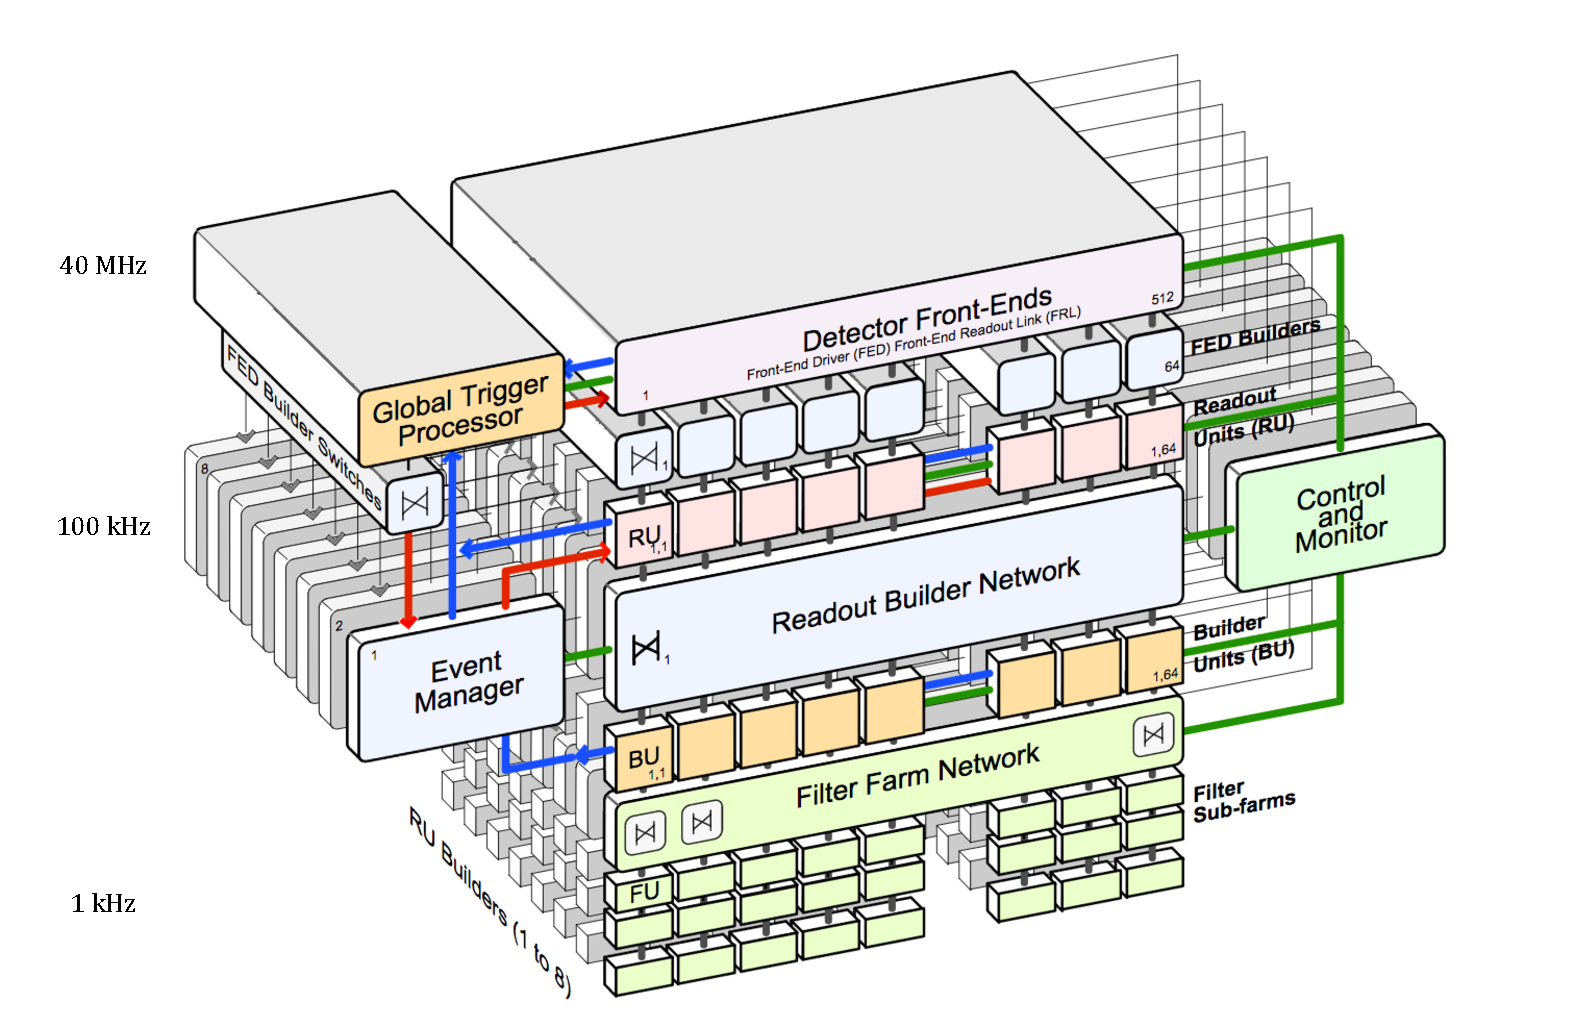
\includegraphics[width=0.9\textwidth]{ch3_figs/cms_daq.pdf}
   \caption{A schematic of the CMS DAQ system.}
   \label{fig:cms_daq}
   %%http://iopscience.iop.org/article/10.1088/1748-0221/3/08/S08004/pdf#%5B%7B%22num%22%3A215%2C%22gen%22%3A0%7D%2C%7B%22name%22%3A%22XYZ%22%7D%2C82.959%2C499.674%2Cnull%5D
 \end{center}
\end{figure}

% % uncomment the following lines,
% if using chapter-wise bibliography
%
% \bibliographystyle{ndnatbib}
% \bibliography{example}
